\documentclass[inf, h]{pjatkThesis}
%
\usepackage{xurl}
\usepackage{float}
%\usepackage{fancyhdr}
%\pagestyle{fancy}
\usepackage{times}
\usepackage[polish,english]{babel}
%
\usepackage{sidecap}
\usepackage{graphicx}
\graphicspath{ {Images/} }
\usepackage{wrapfig}
\usepackage{subcaption}
\newcommand*{\captionsource}[2]{%
  \caption[{#1}]{%
    #1%
    \\\hspace{\linewidth}%
    {Źródło:} #2%
  }%
}
%
\usepackage{makeidx}
\usepackage{xargs} 
\usepackage{lipsum}
\usepackage[pdftex,dvipsnames]{xcolor}
%
%TODO Show \thiswillnotshow notes, remove line below for final version, and review after
%\setlength {\marginparwidth }{2cm}
\usepackage[disable,colorinlistoftodos,prependcaption,textsize=tiny]{todonotes} % use \usepackage[disable]{todonotes} to switch off
\newcommandx{\unsure}[2][1=]{\todo[linecolor=red,backgroundcolor=red!25,bordercolor=red,#1]{#2}}
\newcommandx{\info}[2][1=]{\todo[linecolor=OliveGreen,backgroundcolor=OliveGreen!25,bordercolor=OliveGreen,#1]{#2}}
\newcommandx{\change}[2][1=]{\todo[linecolor=blue,backgroundcolor=blue!25,bordercolor=blue,#1]{#2}}
\newcommandx{\improvement}[2][1=]{\todo[linecolor=Plum,backgroundcolor=Plum!25,bordercolor=Plum,#1]{#2}}
\newcommandx{\thiswillnotshow}[2][1=]{\todo[linecolor=blue,backgroundcolor=blue!25,bordercolor=blue,#1]{#2}}
%
%
\usepackage{listings,xcolor}
%Listings settings
\lstset{
tabsize = 4, 
showstringspaces = false, %% prevent space marking in strings, string is defined as the text that is generally printed directly to the console
numbers = left, 
commentstyle = \color{green}, 
keywordstyle = \color{blue}, 
stringstyle = \color{red}, 
rulecolor = \color{black}, %% set frame color to avoid being affected by text color
basicstyle = \small \ttfamily , %% set listing font and size
breaklines = true, 
numberstyle = \tiny,
}
%
%
%

\author{Kamil Kacprzak}
\album{s14004}
\title{Rozwój technologii wirtualnej rzeczywistości na przykładzie rękawicy-kontrolera}
\type{Praca inżynierska}
\supervisor{dr inż. Michał Tomaszewski}
\location{Warszawa}
\date{Czerwiec, 2020}
%
%
%
\begin{document}
\selectlanguage{polish} 
\tableofcontents
\listoffigures
%\listoftables

\begin{abstract}
%\lipsum
\end{abstract}
\selectlanguage{english} 
\begin{abstract}
%\lipsum
\end{abstract}
 

\selectlanguage{polish} 
\pagenumbering{arabic}
\baselineskip=22pt
\chapter{Wstęp}
\label{ch:wstep}
\change{cel i zarys, wytłumaczenie tytułu}
\chapter{Zagadnienia}
\label{ch:zagadnienia}
Aby zagłębić się w temat rozszerzonej rzeczywistości trzeba przede wszystkim zrozumieć czym jest rzeczywistość oraz zdefiniować pojęcia które są używane z tym zagadnieniem. Oprócz tego zostanie opisana historia powstania wirtualnych światów, dotycząca zarówno pierwszych urządzeń jak i wyobrażenia wirtualnego świata przez twórców filmów, a także zostanie opisany świat wirtualny z którego każdy może skorzystać i to już od wielu lat. W tym rozdziale opisano szczegółowo rozdzielenie różnych rodzajów rzeczywistości oraz na podstawie zebranych danych zostały wysunięte wnioski dotyczące potencjału technologii.

\section{Historia kreowania rzeczywistości}
\label{sec:historia}
Rzeczywistość według słownika jest to coś co istnieje naprawdę, bądź sytuacja lub warunki, w których ktoś żyje, coś się odbywa~\cite{sjp1}. Rozróżnienie tych dwóch definicji jest kluczowe ze względu rozszerzonej rzeczywistości. Rozszerzona rzeczywistość jest to tworzenie nowej formy rzeczywistości poprzez krzyżowanie obiektów rzeczywistych i cyfrowych. Z tego punktu widzenia można zauważyć że według drugiej definicji, rozszerzona rzeczywistość jest częścią rzeczywistości, w szczególności jeśli interakcja pomiędzy światami jest częścią czyjegoś codziennego życia. W przypadku pierwszej definicji, rozróżnienie jest bardziej wyraźne - to o czym mowa musi być prawdziwe, istnieć naprawdę. Z racji tego że na moment pisania tej pracy, integracja pomiędzy światami wirtualnymi oraz rzeczywistymi nie jest wystarczająco komfortowa aby mówić o użytkowaniu jej na równi z światem rzeczywistym, w dalszej części pracy jako rzeczywistość, przyjmuje się pierwszą definicje~\cite{XR}. Typy rozszerzonej rzeczywistości wraz z ich definicjami są przedstawione w sekcji~\ref{sec:rodzaje}, jednak z perspektywy historii, wszystko zaczęło się od jednego typu nazywanego wirtualną rzeczywistością - w skrócie VR (z ang. Virtual Reality). Pierwszym urządzeniem pozwalającym użytkownikowi na zajrzenie do wirtualnego świata, a konkretnie tworzenie złudzenia przebywania w innym miejscy jest Sensorama. Produkt ten został stworzony w 1962 roku przez Mortona Heiliga. Projekt ten powstał przed grafiką komputerową w związku z czym bazował na wyświetlaniu filmów jako obrazu. Zaledwie trzy lata później Ivan Sutheraland nazywany również ojcem grafiki komputerowej, pokazał maszynę do generowania wirtualnej rzeczywistości o nazwie Ultimate Display. Niestety była ona dużych rozmiarów jak i wagi, w związku z czym musiała być przymocowana do sufitu. W 1977 roku postęp technologiczny trwa, rozwijając nie tylko komputery ale także technologię VR - Dan Sandin stworzył pierwszy kontroler pozwalający użytkownikowi na interakcje ze światem wirtualnym w postaci rękawicy. Jest to początek dla projektów prezentowanych w dalszej części tej pracy. Wraz z latami osiemdziesiątymi powstały pierwsze urządzenia typu kinect, czyli pozwalające na kontrolowanie oraz interakcję ze światem przy pomocy kamery śledzącej nasze ciało. Jednak dopiero lata dziewięćdziesiąte pozwoliły na użytek technologii w stopniu wystarczającym aby nadawał się on do użytku w branży rozrywkowej. Wirtualna rzeczywistość przeżywa swój prawdziwy rozkwit po raz pierwszy, a to za sprawą powstania firm produkujących pierwsze gogle i rękawice do  wykorzystania w VR, zaprezentowaniu pierwszego urządzenia dla konsumentów którzy mogli korzystać ze swojego ciała w świecie wirtualnym przy użyciu wielu czujników oraz zakupie limitowanych zestawów, a także odkrycie potencjału przez branże rozrywkową, próbującą wprowadzić na rynek liczne produkty. Wzmożone zainteresowanie przyczyniło się również do powstania wielu filmów związanych z tym tematem co jeszcze bardziej pogłębiło zainteresowanie wśród ludzi. Wyobrażenia z filmów jednak odstają znacząco od możliwości technologicznych, a sam rozwój technologii nie jest tak szybki. Z tego oraz wielu innych powodów zainteresowanie normuje się aż do czasu pojawienia się na rynku Oculus Rift  w 2011 roku, który na nowo intryguje ludzi oraz pogłębia ogólne zainteresowanie technologią VR. Więcej na temat googli Oculus oraz innych urządzeń aktualnie znajdujących się na rynku jest powiedziane w sekcji~\ref{sec:okulary}~\cite{historia}.
  
\section{Wpływ kultury na rozwój technologii}
\label{sec:wplyw}
Od dawna wiadomo że rozwój technologii oraz kultura idą ze sobą w parze. Technologia ma wpływ na twórców oraz artystów, pozwalając im tworzyć nowe, bardziej kreatywne wizje przyszłości, jednocześnie dostarczając lepszych do tego środków, a na podstawie tej twórczości wielu naukowców bazowało się tworząc przełomowe wynalazki, takie jak samo prowadzące się samochody czy telekomunikację cyfrową. Również z technologią VR nie było inaczej. W poniższej sekcji zostanie przedstawione jak twórcy kinematografii prezentowali świat wirtualny, jakie to ma skutki na technologię z której teraz korzystają ludzie a także zostanie pokazany świat wirtualny który był dostępny zanim ludzkość odkryła elektryczność~\cite{wynalazki}.

	\subsection{Kinematografia}
	\label{subsec:kino}
	Wśród pozycji filmowych które zdecydowanie miały wpływ na postrzeganie wirtualnej rzeczywistości znajduję się kilka klasyków. Przede wszystkim warto wspomnieć o filmie \textit{Tron}, który zadebiutował w 1982 roku. Film ten pomimo fabuły ściśle powiązanej z technologią, pokazujący losy programisty przeniesionego do pamięci komputera. Kolejną ważną rolą tego filmu było szerokie zastosowanie grafiki komputerowej. W latach dziewięćdziesiątych wraz z rozpowszechnieniem się technologii, temat VR stał się dużo bardziej popularny co również można zaobserwować na podstawie tworzonych filmów. To właśnie w tym okresie powstały produkcje takie jak \textit{Johnny Mnemonic}, pokazujący możliwość przenoszenia danych przy pomocy umysłu, \textit{Kosiarz umysłów} - czyli ekranizacja powieści Stephena Kinga, w której wygenerowano komputerowo cyberprzestrzeń, pobudzając wyobrażenie zastosowania tej technologii w rzeczywistości i przede wszystkim \textit{Matrix}. Kultowa pozycja pokazująca ludzi zamkniętej w wirtualnej rzeczywistości którzy sami nie są tego świadomi z powodu realizmu który jest prezentowany - czyli dokładnie to co jest założeniem wirtualnej rzeczywistości. W filmach tych prezentuje się wiele metod łączenia umysłów wraz z technologią co nie wątpliwie było inspiracją dla wielu osób~\cite{filmy}. Z nowszych pozycji niewątpliwie należy wspomnieć o filmie \textit{Ready Player One}, który pokazuję wizję wirtualnego świata, realnego lecz jednocześnie z elementami dostępnymi tylko w środowisku wirtualnym. Film ten bazuje na wielu elementach technologicznych  dostępnych w chwili obecnej na rynku, jednak nie zintegrowanych ze sobą a przede wszystkim bez powszechnego dostępu co mogłoby pozwolić na zintegrowanie użytkowników ze światem wirtualnym. Jest on dla wielu wizją tego w jakim kierunku zmierza technologia oraz integracja wielu urządzeń takich jak bieżnie pozwalające na przemieszczanie się w każdym kierunku, realna odczucia całego ciała przy wykorzystaniu odpowiednich kombinezonów no i oczywiście kontrola oraz interakcja przy wykorzystaniu rękawic oraz ciała użytkownika~\cite{p1}. Wszystkie te wizje sprawiają że użytkownicy pragną coraz bardziej realnych doznań oraz interakcji, a także możliwości osiągnięcia wykonania zadania bez konieczności wychodzenia z domu. Oczywiście realizując to, każdy wie że znajduje się w świecie wirtualnym z powodu świadomego przejścia. Gdyby jednak nawet ktoś się obudził w takiej przestrzeni nieświadomy tranzycji pomiędzy rzeczywistościami, łatwo można to określić na podstawie zamontowanych kontrolerów, kombinezonów czy okularów które wyczuwa się na ciele, a także wad elementów graficznych którym wciąż brakuje wystarczającego realizmu. Istnieje jednak metoda która pozwala temu zapobiec, która może posłużyć jako przykład wirtualnego świata w trybie pojedynczego gracza.
	
	\subsection{Marzenia senne}
	\label{subsec:sny}
	Podczas analizy sztucznej rzeczywistości ważnym punktem jest sen, a konkretnie marzenia senne. Przeciętnie człowiek potrzebuje od siedmiu do dziewięciu godzin snu dziennie w cyklu monofazowym, czyli gdy zasypia się i budzi tylko raz dziennie. W tym czasie występują marzenia senna, potocznie nazywane snami. W zależności od osoby swoje sny można pamiętać bądź nie, jednak warto podkreślić że każda osoba ma sny - zapamiętywanie marzeń sennych, tak jak z każdą inną umiejętność można wytrenować, aby pamiętać więcej szczegółów, miejsc oraz wydarzeń. Mając to na uwadze należy sprecyzować czym one właściwie są. Marzenia senne są serią myśli, obrazów oraz odczuć które dana osoba przeżywa w swoim umyśle w trakcie snu. Nie jest to też dowolny moment w trakcie spania. Sen odbywa się w cyklach, które średnio trwają dziewięćdziesiąt minut i składają się z kilku faz takich jak sen przejściowy, głęboki sen czy faza ruchu gałek ocznych - w każdej fazie można śnić jednak to w tej ostatniej najczęściej występują marzenia senne które są rzeczywiste i realistyczne - w wielu przypadkach nie sposób ich odróżnić od rzeczywistości. Faza ta nazywana fazą REM ( z ang. Rapid Eye Movement) jest etapem snu w którym nasz umysł wprowadzany jest w specjalny stan aby móc osiągnąć ten efekt. Przede wszystkim warto zauważyć że etap ten charakteryzuje się wysoką aktywnością mózgu, porównywalną z tą gdy osoba jest przytomna, sprawia to że bardzo łatwo przerwać ten etap i wybudzić się w trakcie snu. Oprócz tego w naszym mózgu przepływa wiele impulsów przez różne jego obszary, niejako testując połączenia, co jest podejrzewane jako przyczynę tworzenia się w naszym umyśle obrazów, doznań dźwiękowych oraz ruchowych. Aby jednak impulsy nie zostały wysłane do mięśni w ciele, w trakcie snu występują ich atonia, czyli zniesienia napięcia mięśniowego. W ten sposób w trakcie gdy ciało leży nieruchomo, w odpowiednim momencie snu dochodzi do symulacji świata w umyśle, w trakcie której osoba może przeżywać wydarzenia które mogą być nawet nie możliwe do zrealizowania w świecie rzeczywistym. Interesującym jest więc fakt, że większość osób zdaje sobie sprawę tuż po przebudzeniu, że wydarzenia które przed chwilą miały miejsce były jedynie marzeniami sennymi - nie były one rzeczywistością. Dzieje się tak za sprawą kory przedczołowej - części mózgu która jest odpowiedzialna za myślenie logiczne, planowanie ruchów i działań, oraz pełni funkcje w działaniu pamięci roboczej. Kora przedczołowa jest jednym z obszarów mózgu który w trakcie snu wytwarza jedynie minimalną aktywność co sprawia że gdy marzenia senne zaczynają się w zupełnie innym miejscu od lokalizacji danej osoby, z ludźmi których dana osoba nie zna, bądź wręcz nie powinno ich tam być, jak na przykład osoby zmarłe bądź znajdujące się w innym miejscu na ziemi, mózg tego nie kwestionuje - przyjmuje że to co się dzieje jest zupełnie normalne. Za sprawą tych mechanizmów, niejako każda osoba codziennie ma dostęp to sztucznej rzeczywistości w której może znaleźć się w dowolnym miejscu, z dowolnymi osobami, przeżywając zdarzenia które mogą być nawet sprzeczne z prawami fizyki. 
	
W obecnych czasach jeżeli mówimy o wirtualnej rzeczywistości, nie myślimy o maszynie takiej jak Sensorama, która jedynie wyświetlała filmy. Poruszając ten temat myślimy o kontrolowanym środowisku w którym użytkownik ma możliwość interakcji z otoczeniem a nawet jego kontrole. W rozumieniu marzeń sennych, zwykłe sny są tym czym Sensoroma jest dla współczesnej technologii VR. Świadome śnienie natomiast odkrywa pełną moc możliwości która kryje się w tym naturalnym ludzkim procesie. Aby podjąć próbę świadomego snu należy oczywiście najpierw być w stanie pamiętać swoje zwyczajne marzenia senne. Świadomy sen jest to rodzaj snu w którym osoba śniąca zdaje sobie sprawę z tego że znajduje się w świecie marzenia sennego. Istnieje wiele metod które pozwalają osiągnąć ten stan, jednak ogólnie mówiąc sprowadzają się one do kwestionowania rzeczywistości, dzięki czemu możemy niejako zakodować ten proces w podświadomości. Tak jak wspomniano kora przedczołowa odpowiadająca za logiczne myślenie nie wykazuje dużej aktywności w trakcie snu, jednak nie jest ona całkowicie nieaktywna, dzięki czemu nadal można ją wykorzystać nawet podczas snu. Jeżeli osoba zakwestionuje rzeczywistość w trakcie marzenia sennego, na przykład poprzez złamanie praw fizyki, i rezultat takiego testu pokaże niemożliwe rezultaty w świecie rzeczywistym, osoba taka odzyskuje świadomość. Często w początkowych próbach dochodzi w tym momencie do wybudzenia, ponieważ jest to niejako przełamanie naturalnego mechanizmu organizmu. Z praktyką jednak dochodzi do stabilizacji świata a dzięki uzyskaniu świadomości, dochodzi do uzyskania kontroli nad naszym umysłem, czyli marzeniem sennym. W ten oto sposób mózg od wewnątrz, bez dodatkowych urządzeń i kontrolerów, generuje własny świat ''wirtualny``, odtwarzając bodźce wzrokowe, słuchowe, dotyku oraz wszystkie inne zmysły. Osoba kontrolująca ma pełną kontrole nad własnym ciałem i z jej perspektywy świat w którym się znajduje dostarcza tych samych bodźców co świat rzeczywisty, a dla osób które potrafią kontrolować otoczenie, bodźców możliwych do doświadczenia jedynie poza światem rzeczywistym takich jak np. latanie czy teleportacja~\cite{sen2}~\cite{sen1}. 		
	
\section{Rodzaje rzeczywistości}
\label{sec:rodzaje}
Umiejętność świadomego snu jest treningiem przejęcia kontroli nad naturalnym procesem śnienia występującym u każdej osoby, pozwalając niejako doświadczyć tego dokąd technologia wirtualnej rzeczywistości zmierza - bezbłędnego odwzorowania świata rzeczywistego, przy dostarczeniu do mózgu wszystkich bodźców w taki sposób aby osoba użytkująca odniosła pełne wrażenie realizmu otoczenia. Mając to na uwadze, w tej sekcji zostanie zdefiniowane czym jest rozszerzona rzeczywistość, jakie rodzaje rzeczywistości obejmuje ten termin oraz wyjaśnić dokładnie pojęcie wirtualnej rzeczywistości które było używane w tym rozdziale. 
	%\subsection{XR}
%	\label{subsec:xr}

	Akronim XR (z ang. Extended Reality) jest tłumaczony na język polski na wiele sposobów takich jak rzeczywistość rozszerzona ( w odróżnieniu od rozszerzonej rzeczywistości) czy rzeczywistość skrzyżowana. W praktyce jednak najczęściej używa się skrótów angielskich które pozwalają jednoznacznie określić zagadnienie. Termin XR jest używany jako ogólne wyrażenie wszystkich technologii wpływających na zmianę rzeczywistości, które mogą zostać użyte razem bądź pojedynczo. W związku z tym aplikacje mieszające obiekty wirtualne z rzeczywistymi które mogą dowolnie przełączać się pomiędzy tym światem a światem czysto wirtualnym są określane tym terminem, jak i każdy z projektów wykorzystujących tylko jeden typ technologii zmiany rzeczywistości. W chwili pisania tej pracy terminem XR określa się zbiór technologi wirtualnej rzeczywistości, rozszerzonej rzeczywistości a także mieszanej rzeczywistości, jednak określenie to powstało w celu włączenia do jednego określenia również wszystkich terminów które mogą zostać stworzone w przyszłości~\cite{terms}.
	%\subsection{VR}
	%\label{subsec:vr}
	
	Pojęcie wirtualnej rzeczywistości określa się skrótem VR ( z ang. Virtual Reality) i definiuje ono część technologii kreowania rzeczywistości w pełni wirtualnej - oznacza to że nie znajdują się w niej żadne elementy świata rzeczywistego. Jeżeli elementy te miały by być prezentowane w takim środowisku muszą one zostać wygenerowane komputerowo. Celem VR jest stworzenie jak najbardziej realistycznych i rzeczywistych odczuć dla użytkownika niezależnie od środowiska w jakim się znajduje. Aby to osiągnąć niezbędna jest symulacja która wpływa na wszystkie zmysły użytkownika. Dlatego też firmy pracują nad coraz bardziej realistycznymi i dokładnymi rozwiązaniami które pozwalają na głębszą imersję w świat wirtualny. Jest to również jednym z głównych powodów dla których zostały stworzone rękawice-kontrolery. Pozwalają one na większą swobodę oraz bardziej naturalny ruch w  wygenerowanej przestrzeni, zapewniając lepsze odczucia oraz komfort podczas przebywania w świecie wirtualnym. Nad zapewnieniem realizmu, oprócz metody kontroli środowiska, składa się wiele innych czynników. W tym celu powstają specjalne kombinezony które odwzorowują ruch całego ciała, bieżnie które pozwalają się poruszać w VR, dzięki naturalnemu przemieszczeniu się, które za sprawą bieżni odbywa się w miejscu w świecie rzeczywistym, okularów które pozwalają wyświetlać przed oczami środowisko wirtualne, starając się odwzorować głębię oraz wiele innych urządzeń. Ilość urządzeń oraz metod imitacji pokazuje jak skomplikowanym problemem jest odwzorowanie rzeczywistości, a wszystko to musi odbywać się niezwykle płynnie ponieważ mózg człowieka nie rozróżnia rzeczywistości od świata wirtualnego. Oznacza to że jeżeli bodźce wzrokowe nie pokrywają się z bodźcami słuchowymi dochodzi do tak zwanego zjawiska choroby lokomocyjnej. Sprawia to że przebywania w wirtualnym świecie przez długi okres czasu może doprowadzić do dyskomfortu dla użytkownika. Aby zapobiec tego rodzaju problemom równie ważnym jest dokładna znajomość fizjologii człowieka, co prowadzi do współpracy wielu działów nauki w celu stworzenia prawdziwie realistycznych produktów. Pomimo wielu przeszkód jak przedstawiono w sekcji~\ref{sec:historia}, wirtualna rzeczywistość była pierwszą wizją naukowców którą starano się zrealizować - pomimo dużych nakładów pracy w celu zapewnienia realistyczności, niesie ona za sobą wiele możliwości zarówno w biznesie jak i życiu codziennym, co sprawia że dla wielu firm jest to możliwość realizowania własnej wizji wirtualnej przyszłości~\cite{terms}~\cite{chorobaVR}.
	%\subsection{AR}
	%\label{subsec:ar}
	
	Kolejnym terminem wchodzącym w skład XR jest rozszerzona rzeczywistość, bądź też nazywana rzeczywistością poszerzoną. Skrótowo zapisuje się ją jako AR (z ang. Augmented Reality). Podobnie brzmiąca do XR w szczególności w języku polskim jest częstym powodem dla którego powszechnie używa się skrótów angielskich mówiąc o tym obszarze technologii. AR jak nazwa wskazuje poszerza rzeczywistość zamiast ją zastępować tak jak to miało w przypadku VR. Oznacza to że do elementów świata rzeczywistego zazwyczaj pozyskanych przy pomocy obrazu z kamery, wyświetlanych poprzez wybrane źródło obrazu o których mowa w rozdziale~\ref{ch:prezentacja}, są dodawane elementy stworzone przy pomocy grafiki komputerowej, zazwyczaj trójwymiarowe. Technologia ta dzięki wykorzystaniu w dużej mierze świata rzeczywistego jest łatwiejsza w użytkowaniu a jej zastosowanie jest powszechnie stosowane w wielu branżach. W szczególności duży sukces technologia ta odniosła gdy wykorzystano ją do stworzenia popularnej gry na smart-fony \textit{Pokemon Go}, która przy wykorzystaniu geolokalizacji oraz AR zapewniała realistyczne doświadczenia łapania stworzonych trójwymiarowych postaci w świecie rzeczywistym~\cite{terms}. Podgląd interfejsu aplikacji obrazujący wykorzystanie technologii AR  w \textit{Pokemon Go} pokazuje rysunek~\ref{fig:pokemon}.
	
\begin{figure}[h]
\centering
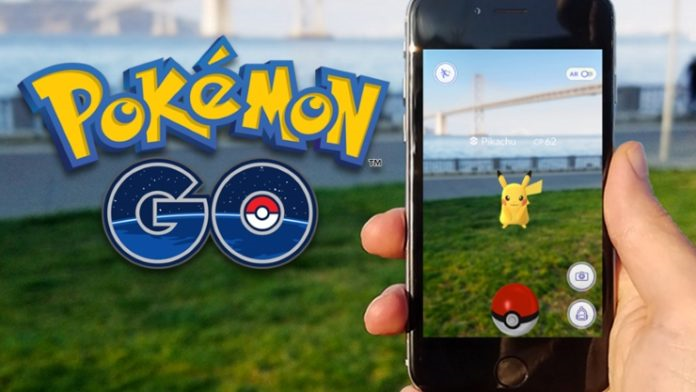
\includegraphics[scale=0.6]{pokemon}
\captionsource{Interfejs aplikacji \textit{Pokemon Go} wykorzystujący AR.}{\url{https://gameradar.pl/aktualizacja-pokemon-go-utrudnia-lapanie-pokemonow/}}
\label{fig:pokemon}
\end{figure}

	%\subsection{MR}
	%\label{subsec:mr}	
	
	Mieszana rzeczywistość, czyli MR (z ang. Mixed Reality) jest terminem który prawdopodobnie jest najczęściej błędnie używanym wśród zagadnień związanych z XR. Mieszana rzeczywistość podobnie jak AR wykorzystuje do działania zarówno świat rzeczywisty jak i stworzony komputerowo, jednak w odróżnieniu od AR nastawiony jest głównie na interakcję pomiędzy tymi światami. Obiekty tworzone cyfrowo wyświetlane w świecie rzeczywistym mogą być modyfikowane i wpływać na środowisko rzeczywiste które jest wyświetlane jak i obiekty rzeczywiste mogą zostać przeniesione do świata wirtualnego. Interakcja ta i zastosowanie jest niejako technologią przyszłości, wizją producentów, ponieważ do tej pory nie ma łatwo dostępnych produktów które by wykorzystywało ten rodzaj XR, natomiast istnieją takie rozwiązania dla biznesu oraz w ośrodkach badawczych, które prawdopodobnie staną sie bardziej dostępne wraz z rozwojem tej technologii oraz ulepszonych rozwiązań w innych dziedzinach technologicznych takich jak grafika komputerowa, prędkość przesyłania czy przetwarzania danych~\cite{terms}.
%\section{Potencjał technologii}
%\label{sec:potencjal}

Rozwiązania XR przebyły długą drogę od czasu powstania pierwszej wizji tego typu rozwiązania. Obecnie istnieje wiele urządzeń które powszechnie korzystają z XR zarówno na użytek prywatny, branży rozrywkowej oraz w celu usprawnienia procesów biznesowych. Niemniej jednak dopiero są opracowywane rozwiązania które mogłyby zapewnić większą przenośność tego typu urządzeń, sprawniejsze połączenie i przede wszystkim realizm. Wykorzystanie w życiu codziennym staje się coraz bardziej powszechne, w związku z tym można też się  spodziewać ulepszeń produktów zarówno pod względem sprzętu jak i oprogramowania a także dostępności tych produktów przy mniejszym koszcie. Można być pewnym że technologia ta nie przestanie się rozwijać, znajdując coraz to nowe zastosowania, inwestorów a także twórców którzy wprowadzając większą liczbę produktów na rynek, tworzą większe zainteresowanie wśród społeczności. Pytanie stawiane przez technologię XR to nie czy ta technologia ma przyszłość, a kiedy stanie się ona powszechnie stosowana. W dalszych częściach tej pracy zostaną pokazane sposoby w jakich obecnie przedstawiane i wykorzystywane są opisywana do tej pory technologie, a także zostanie szczegółowo opisany temat rękawic-kontrolerów, urządzenia które nie jest standardem wśród kontrolerów na rynku dla pojedynczych konsumentów VR, jednak już jest wykorzystywany w biznesie a także przewidywany jest jako kontroler przyszłości~\cite{terms}.


\chapter{Komponenty rękawicy-kontrolera}
\label{ch:komponenty}
\change{Opis rękawic na rynku}

	\section{Nawigacja inercyjna}
	\label{sec:inercja}
	\change{INS - inertial navigation system}
	\change{Jak dostępne rękawice omijają problem}

	
	
	\section{IMU - Inercyjna jednostka pomiarowa}
	\label{sec:imu}
	
		\subsection{Żyroskop}
		\label{subsec:gyro}
		
		\subsection{Akcelerometr}
		\label{subsec:acc}
		
		\subsection{Magnetometr}
		\label{subsec:mag}
	
	\section{Stopnie swobody}
	\label{sec:swobody}	
	%TODO Gimbal lock
	
\section{Porównanie Bluetooth z BLE(z ang. Bluetooth Low Energy)}
\label{sec:bvsble}
\improvement{TODO: BLE section}
\change{UUID section?}
tak zwany uniwersalny unikalny identyfikator znany pod akronimem UUID (z ang. Universally Unique IDentifier). 
	
	\section{Monitorowanie położenia palców}
	\label{sec:palce}
	
\chapter{Projekt rękawicy}
\label{ch:rekawica}
Istotą poniższego rozdziału jest pokazanie użytych w projekcie podzespołów i technologii oraz lepsze zrozumienie powodów dla których to właśnie te produkty zostały wybrane. Po zapoznaniu się z motywem, zostanie szczegółowo opisana specyfikacja tych produktów a także sposób ich poskładania w spójną całość, co sprawiło pewne problemy względem oryginalnego szkicu - próby oraz efekty rozwiązywania tych problemów również zostaną opisane w tym rozdziale. Po nakreśleniu podstawowych założeń projektu zostanie zaprezentowana finałowa wersja, a także szczegółowo zostanie omówiony kod rękawicy-kontrolera, który jest obsługiwany przez mikrokontroler i stanowi najważniejszą część tego projektu.\improvement{Następny rozdział?} Po zaznajomieniu się z kodem aplikacji, będą zaprezentowane wady oraz możliwe ulepszenia projektu, jakie ukazały się w trakcie prac nad aplikacją obsługującą i wykorzystującą dane z rękawicy, w celu ich prezentacji o czym będzie więcej mowa w rozdziale~\ref{ch:aplikacja} dotyczącym tejże właśnie aplikacji.

\section{Przegląd podzespołów użytych w projekcie}
\label{sec:przeglad}
Jak dowiedzieliśmy się z rozdziału \ref{ch:komponenty} dotyczącego podstawowych komponentów rękawic, kluczowym dla powodzenia projektu jest ustalenie następujących pozycji: 
\begin{itemize}
\item orientacji dłoni względem punktu początkowego
\item położenia względem punktu początkowego
\item moment i stopień zgięcia palców 
\end{itemize}
 W tym celu należy zebrać informacje z czujników, a następnie wszystkie te informacje należy przesłać do pożądanego urządzenia. Elementem które pozwala to osiągnąć w tym projekcie jest mikrokontroler Arduino nano 33 BLE, który odpowiada za dostarczenie informacji z żyroskopu, akcelerometru a także czujników wygięcia. Zasady działania pierwszych dwóch zostały opisane z podrozdziałach~\ref{subsec:gyro} oraz ~\ref{subsec:acc}. Natomiast w poniższych podrozdziałach zostanie opisane rozwiązanie zastosowane do odczytu położenia palców, zasada działania przy wykorzystaniu rezystorów oraz sposób połączenia wszystkich wspomnianych elementów w jeden finałowy kontroler.
	
	
	\subsection{Mikrokontroler}
	\label{subsec:arduino}
	Jak przed chwilą wspomniano, w projekcie wykorzystywana jest płytka od Arduino, która nosi nazwę Nano 33 BLE. Jest to małych rozmiarów płytka o  wymiarach 45 x 18 mm, pozwalająca na wysoką wydajność przy jednoczesnym małym poborze prądu, co zapewnia użyty mikrokontroler nRF52480 o taktowaniu 64 MHz. Do dyspozycji mamy również pamięć RAM o pojemności 256 kB oraz pamięć Flash o pojemności 1 MB. IMU które zostało zamontowane na płytce to LSM9DS1, które obsługuję akcelerometr, żyroskop oraz magnetometr w trzech osiach. Więcej infomracji na temat IMU jest przedstawione w części~\ref{sec:oprogramowanie}. Warto na wstępie zauważyć że Nano 33 BLE pracuje domyślnie wyłącznie z napięciem 3,3 V, w związku z czym nie należy podłączać bezpośrednio zasilania o większym napięciu. W celu podłączenia zasilania 5 V należy zlutować zworkę znajdującą się pomiędzy pinami RDT oraz A7 - temat ten nie zostaje jednak poruszony w tej pracy, ponieważ na potrzeby projektu używane jest zasilanie poprzez złącze micro USB które to również jest obsługiwane. Płytka ta posiada wiele użytecznych sensorów, jednak na potrzeby tej pracy została wybrana z powodu wbudowanej inercyjnej jednostki pomiarowej, dzięki czemu można było uprościć konstrukcję   oraz zmniejszyć ilość połączeń na rękawicy, wbudowanego modułu Bluetooth - a w tym przypadku modułu Bluetooth Low Energy obsługiwanego w standardzie 5.0, a to wszystko w przystępnej cenie co również było jednym z kryteriów przy tworzeniu tego projektu. Płytkę w momencie tworzenia tej pracy można kupić za 119 zł. Wartym uwagi jest fakt możliwości zakupu płytki bez wyprowadzonych złącz, co w przypadku opisywanego projektu pozwoli na zmniejszenie wymiarów oraz większą swobodę montażu.~\cite{botland-arduino}
	
	Z najważniejszych elementów układu płytki należy wiedzieć że posiada ona dwie diody po dwóch stronach portu micro USB - zielona indykuje podłączone zasilanie, natomiast pomarańczowa zaczyna mrugać gdy jest przesyłany kod do mikrokontrolera. Oprócz tego do dyspozycji są dwa piny wyjściowe zasilające o napięciu 3,3 V oraz 5 V, jeden pin zasilający wejściowy, którego ograniczenia zostały wspomniane w poprzednim paragrafie, a także dwa piny uziemiające, po jednym z każdej strony płytki. Posiada ona piny zarówno analogowe jak i cyfrowe, jednak na potrzeby tego projektu zostały użyte jedynie piny analogowe, których do dyspozycji jest aż osiem umiejscowionych po jednej stronie, przy czym warto zwrócić uwagę że piny A4 oraz A5 używane są jako magistrala I2C w związku z czym zalecane jest nie stosowanie tych wejść analogowych. Szczegółowy opis wejść/wyjść płytki przedstawiony jest na grafice~\ref{fig:arduino}.
	
\begin{figure}[h]
\centering
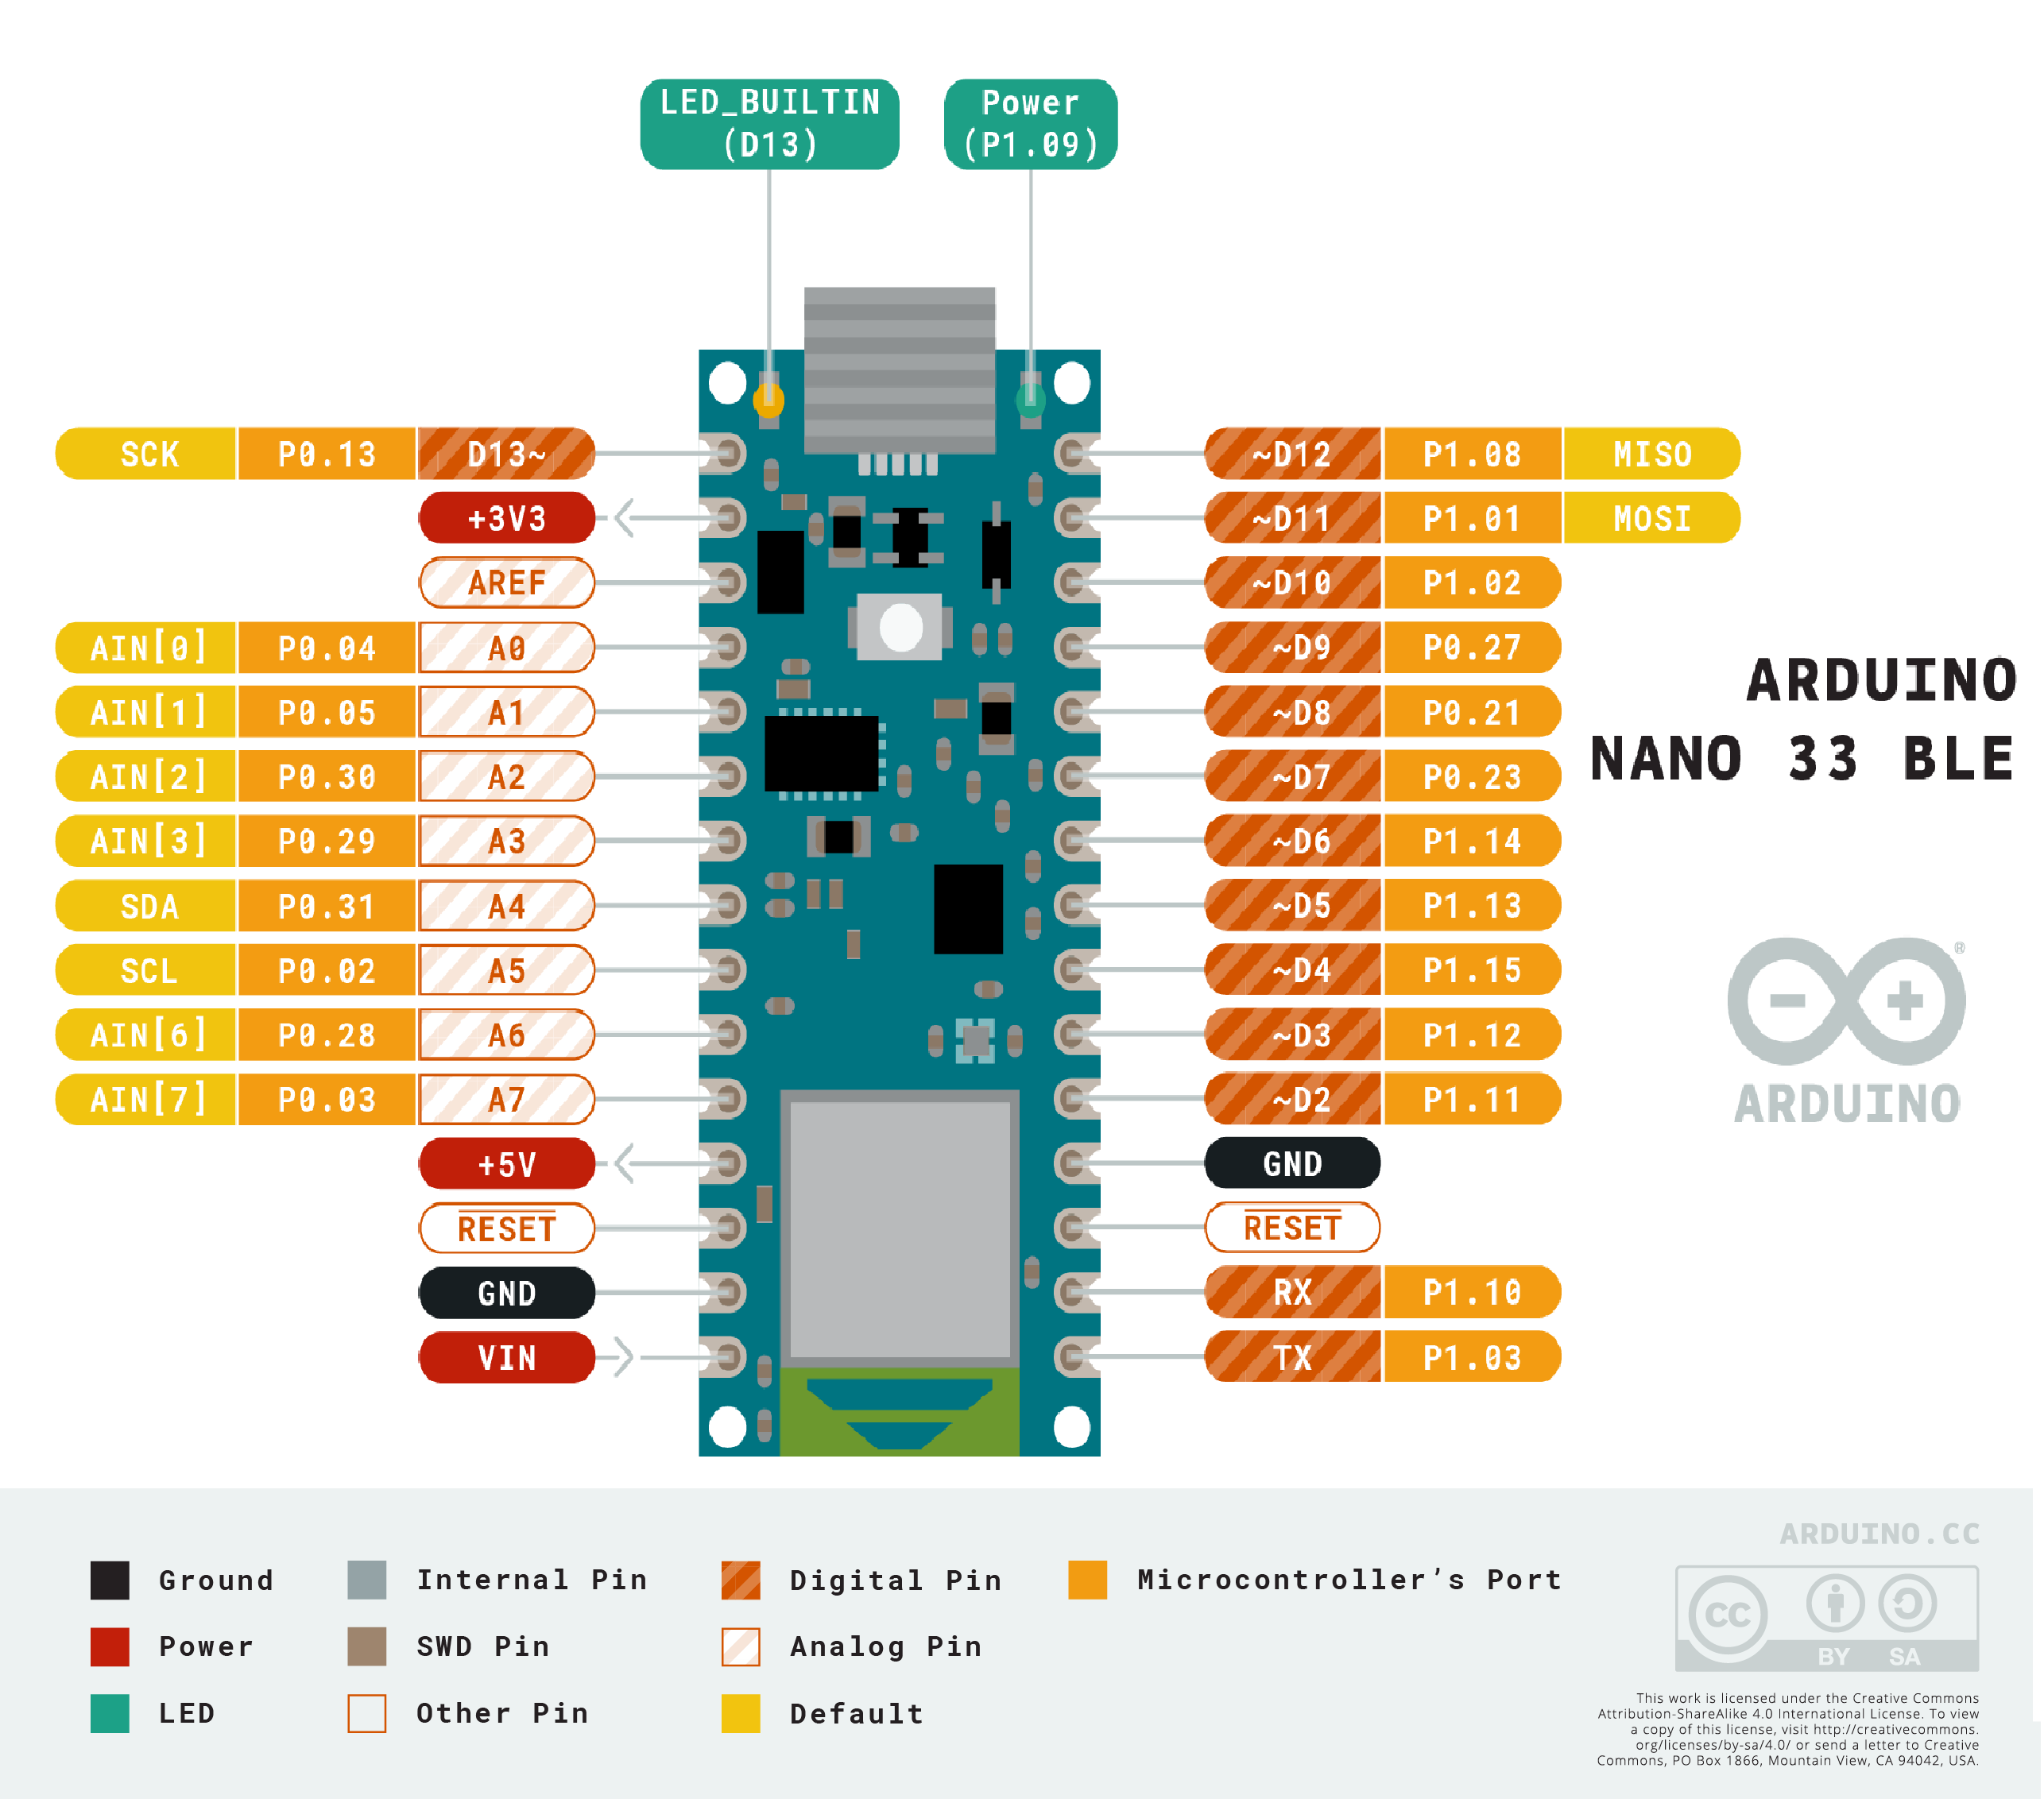
\includegraphics[scale=0.5]{arduino}
\captionsource{Opis wejść oraz wyjść Arduino Nano 33 BLE}{\url{https://content.arduino.cc/assets/Pinout-NANOble_latest.pdf}}
\label{fig:arduino}
\end{figure}

	W tym projekcie wykorzystano zasilanie poprzez złącze micro USB, wyjście o napięciu 3,3 V w celu uzyskania odczytów z czujników wygięcia na pinach analogowych A0, A1, A3, A6 oraz A7, o których zostanie więcej powiedziane w punkcie~\ref{sec:budowa}, a także uziemienie znajdujące się po tej samej stronie płytki.

	\subsection{Czujnik wygięcia}
	\label{subsec:wygiecie}	
	Kluczowym dla działania kontrolera jest możliwość określenia pozycji palców względem dłoni. Ma to wiele zastosowań zarówno wizualnych jak i praktycznych. Ważne jest aby odwzorować świat rzeczywisty tak dokładnie jak to możliwe - im lepsze odwzorowanie tym bardziej zmysły użytkownika zostaną oszukane, podwyższając komfort użytkowania technologii wirtualnej rzeczywistości. Za stroną praktyczną natomiast przemawia możliwość śledzenia palców w celu dokładnego ich użycia w stworzonym środowisku np. do ściskania i podnoszenia obiektów czy też korzystania z klawiatury wirtualnej. Jak wspomniano w rozdziale~\ref{ch:komponenty} dotyczącym komponentów komercyjnych rękawic - wśród znanych producentów na rynku, decyduję się na użycie wielu inercyjnych jednostek pomiarowych, na podstawie których są w stanie dokładnie określić położenia każdej części palca, bądź też nie aż tak popularne rozwiązanie, które wykorzystujące specjalistyczne sensory służące do pomiaru stopnia wygięcia czujnika względem pozycji prostej.
Czujnik ten po podłączeniu do prądu zwiększa swój opór wraz ze zwiększonym stopniem odchylenia. Oba te rozwiązania pomimo wysokiej dokładności pomiarów nie są rozwiązaniami tanimi. W związku z tym na potrzeby stworzenia taniego kontrolera, należało znaleźć rozwiązanie bardziej przystępna a jednocześnie pozwalające na osiągnięcie tego samego celu.
	
	Aby osiągnąć postawione założenia zostały skonstruowane czujniki wygięcia w domowych warunkach. Rozwiązanie to jest często używane do osiągnięcia pomiaru stopnia wygięcia bez konieczności wydawania ponad 100 zł na jeden czujnik~\cite{flex-sensor}. Jest ono stosunkowo proste w założeniach i wymaga jedynie dwóch kluczowych elementów. Tkaniny przewodzącej o specjalnych właściwościach oraz dwóch przewodników po obu stronach materiału. Z jednej strony zostanie podłączone napięcie z drugiej natomiast uziemienie. Ważnym jest aby połączenia te się ze sobą nie stykały w żadnym punkcie a jedynie zostały nałożone na siebie, z tkaniną ściśniętą pomiędzy nimi - dzięki temu mamy pewność że odczyty które otrzymamy będą prawidłowe. Pozostaje odpowiedzieć na pytanie jakiego rodzaju materiał należy wykorzystać. Na rynku znajdziemy wiele rodzajów materiałów które zmieniają swój opór w zależności od spełnienia takich kryteriów jak nacisk, temperatura, rozciągnięcie czy też właśnie zgięcie materiału. Pomimo próby uzyskania materiału który zmienia swój opór w zależności od rozciągnięcia, co pozwoliłoby na skonstruowanie części na palce rękawiczki z tego materiału, zapewniając dokładniejszy i bardziej estetyczny efekt końcowy, w momencie projektowania rękawicy był on jedynie możliwy do sprowadzenia ze stanów, co nie było najtańszym rozwiązaniem. W związku z tym zdecydowano się na użycie foli Velostat która jest czuła na nacisk or zginanie~\cite{velostat}. W roli przewodnika wybrano nić przewodzącą, która zapewniła potrzebną elastyczność oraz możliwość przymocowania poszczególnych elementów przy jednoczesnym zapewnieniu funkcjonalności. Elementy te zostały sklejone na kawałku taśmy samoprzylepnej oraz dodatkowo sklejone przy brzegu aby nić nie wyśliznęła się w trakcie korzystania z czujnika. Efekt końcowy jest widoczny na zdjęciu~\ref{fig:sensor}. W celu otrzymania pomiarów wszystkich palców zostało wykonanych pięć takich sensorów, o szerokości 15 mm; dwa o długości 8 cm, dwa o długości 10 cm a także jeden 11 cm, w celu jak najlepszego dopasowania względem miejsca na palce na zakupionej rękawicy do której sensory zostaną przymocowane, co można zobaczyć na zdjęciu~\ref{fig:glove}.
	
\begin{figure}[h]
\centering
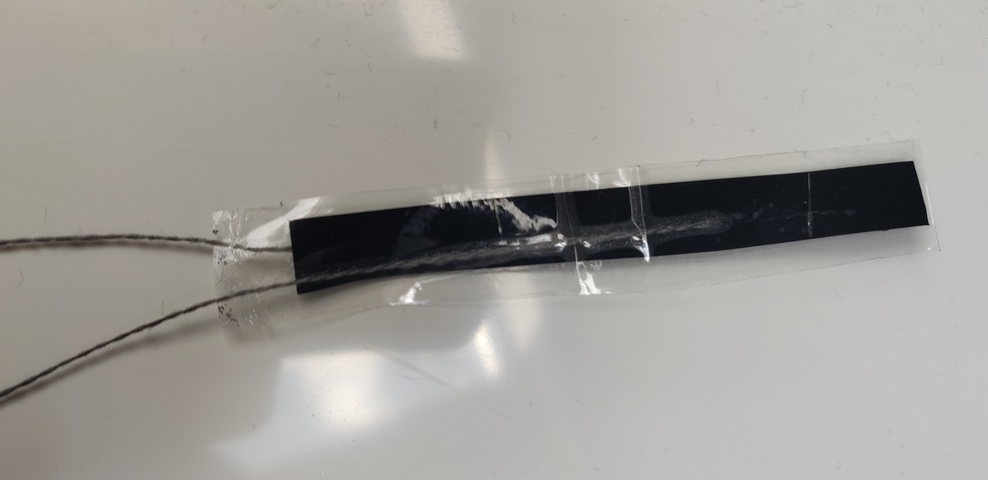
\includegraphics[scale=0.65,width=\textwidth]{flex-sensor}
\caption{Sensor wygięcia własnego wykonania}
\label{fig:sensor}
\end{figure}	

	\subsection{Rezystor}
	\label{subsec:rezystor}	
	Rezystor, potocznie zwany opornikiem, jest to prosty element elektroniczny, posiadający jedynie wyjścia z dwóch stron elementu łączącego. Element ten tworzy opór, powodując ograniczenie przepływającego przez niego prądu gdy jest włączony do obwodu szeregowo. Opór ten jest mierzony w omach. Istotną informacją jest fakt że nadmiar prądu jest zamieniany przez opornik na energie cieplną, a także brak zdefiniowanego kierunku - co oznacza że działa on niezależnie od sposoby zanotowania go w układzie.
	
	Pomimo swojej prostoty budowy i zastosowania, dla danego projektu ważne jest aby wybrać odpowiednie rezystory. Podstawową wartością na którą należy zwrócić uwagę jest rezystancja. Rezystancję podaje się w omach i można spotkać na rynku zakres od miliomów do megaomów. Spośród dostępnych rodzajów rezystorów w projekcie zostały użyte rezystory THT ( z ang. Through-Hole Technology) - czyli tak zwane rezystory do montażu przewlekanego. W tym rodzaju oporników rezystancja jest ilustrowana poprzez kolorowe paski umieszczone wokół oporu, co pozwala odczytać ich wartość według ilustracji~\ref{fig:oporniki}. Alternatywą do tego sposobu jest podłączenie rezystora pod miernik elektryczny ustawiony w tryb pomiaru oporu~\cite{rezystor}. 
		
\begin{figure}[h]
\centering
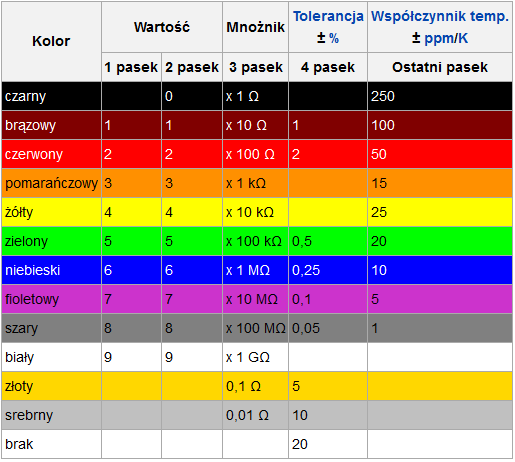
\includegraphics[scale=0.65]{oporniki}
\captionsource{Oznaczenia rezystorów}{\url{https://sites.google.com/site/informatykaunijna/home/poszczegolne-czesci/rezystor}}
\label{fig:oporniki}
\end{figure}
	
\begin{wrapfigure}{l}{0.5\textwidth}
\begin{center}
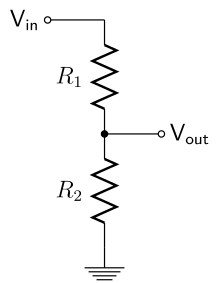
\includegraphics[width=0.48\textwidth]{v-divider}
\captionsource{Układ dzielnika napięcia}{\url{https://www.wikiwand.com/en/Voltage_divider}}
\label{fig:divider}
\end{center}
\end{wrapfigure}

	Element ten jest kluczowy w celu ograniczenia przepływu prądu w obwodzie rękawicy, co pozwala na monitorowanie oporu wytwarzanego poprzez czujnik wygięcia. Sposób działania układu, nazywanego dzielnikiem napięcia jest pokazany na rysunku~\ref{fig:divider}, oraz wyraża się wzorem
	$$
		\nu_{out} = \nu_{in}\left[ \frac{R_2}{R_1+R_2}\right]
	$$
Wzór ten podaje napięcie wyjściowe $\nu_{out}$, które równa się napięciu wejściowemu $\nu_{in}$ przeskalowanemu przez stosunek rezystorów. W opisywanym przypadku jest to stosunek zastosowanego rezystora $4.7 k\Omega$ wyrażonego we wzorze poprzez $R_2$, do sumy tego rezystora wraz z oporem wytwarzanym poprzez czujnik wygięcia $R_1$ - który jak opisano w podrozdziale~\ref{subsec:wygiecie} jest zmienny. Oznacza to że im bardziej czujnik wygięcia jest zgięty, wytwarza on większy opór a co za tym idzie napięcie wyjściowe spada. Miara ta obrazuje jak bardzo palec jest zgięty i jest możliwa do uzyskania właśnie dzięki zastosowaniu układu dzielnika napięcia~\cite{v-divider}.


\section{Budowa rękawicy}
\label{sec:budowa}

W poniższej sekcji zaprezentowano sposób w jaki zostały złączone wszystkie elementy rękawicy wspomniane w sekcji~\ref{sec:przeglad}, aby była gotowa na oprogramowanie mikrokontrolera tworząc finałowy produkt. W tym celu została wybrana rękawica budowlana o grubych niciach ze ściągaczem wokół nadgarstka w celu zapewnienia komfortu, jak i precyzji położenia. Wybór ten również jest uzasadniony faktem początkowego planu dotyczącego wszycia materiału bezpośrednio w rękawice jak i elastyczności które zapewnia grubsza rękawica. Tak jak wspomniano w podsekcji~\ref{subsec:wygiecie}, do połączenia elementów została wykorzystana nić przewodząca. Dzięki grubym włóknom odstępu pomiędzy nićmi przewodzącymi prąd mogły być mniejsze, bez obawy przed spięciami w trakcie poruszania ręką. Dla tego projektu kontroler jest budowany dla lewej dłoni. Układ przewodów kontrolera jest zobrazowany na rysunku~\ref{fig:circuit}. Jest to jedynie obraz poglądowy, przedstawiony na płytce prototypowej a szczegółowy opis połączeń kontrolera zostanie opisany poniżej.

\begin{figure}[h]
\centering
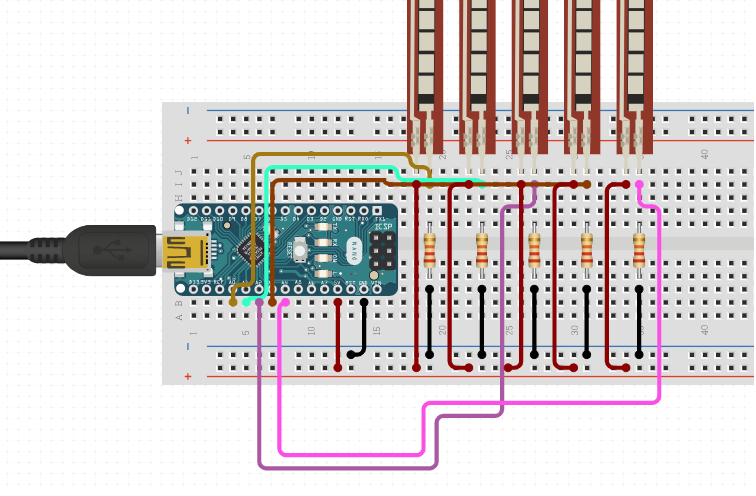
\includegraphics[width=\textwidth]{circuit}
\captionsource{Poglądowy układ kontrolera przedstawiający sposób podłączenia dzielnika napięcia}{\url{https://www.circuito.io/app?components=514,8606,8606,8606,8606,11022}}
\label{fig:circuit}
\end{figure}

Mikroprocesor został umieszczony na wysokości centralnej części dłoni, przy kciuku, skierowany złączem USB na zewnątrz, pozwalając na łatwe podłączenie przewodu zasilającego jak i również ustawienie wejść analogowych w stronę palców lewej dłoni. Z tej strony płytki Arduino będziemy też korzystać - zarówno przy wyprowadzaniu napięcia jak i uziemienia. Montaż samej płytki nie stanowi żadnego problemu ze względy na cztery otwory w rogach pozwalające na mocowanie, do którego została użyta zwykła nić do szycia. Aby stworzyć obwód wychodzący od pinu GND (z ang. Ground) czyli właśnie uziemienia, należy najpierw poprowadzić go przez rezystory. W tym celu wyjścia oporników zostały wygięte w pętle oraz zalutowane aby w łatwy sposób można było je przyszyć do rękawicy. Aby dodatkowo ułatwić sobie to zadanie - dodatkowo zostały one przyklejone bezpośrednio do materiału na bardzo małą ilość kleju. Umiejscowienie rezystorów jest po zewnętrznej wierzchniej stronie dłoni, zaczynając się na wysokości kontrolera, zmierzając szeregowo w stronę nadgarstka. W ten oto sposób nić przewodząca została poprowadzona na zewnętrzną część dłoni a następnie poprzez wszystkie pętle rezystorów, kończąc na ostatnim. Z drugiej strony rezystora dochodzi natomiast nić pochodząca z czujnika oporu. W tym celu podczas tworzenia czujników oporu pozostawiono 25 cm długości nici, co pozwoliło na przymocowanie sensorów, a następnie połączenie obwodu. Sensory zostały zaopatrzone w krótkie, 1-2 cm długości kawałki taśmy elastycznej która została przyklejona na czubku każdego z sensorów pozwalając na elastyczny ruch sensora bez zerwania nici. Taśma ta została przyszyta w czubkach palców co dało punkt zaczepu dla sensorów. W tym momencie pozwoliło to na wygodne używanie nici wychodzących z sensorów w celu zamknięcia obwodu. Z powodu dużego zagęszczenia nici, które nie mogą się ze sobą stykać podczas ruchu ręki, ważnym dla projektu było naprzemienne używanie przestrzeni na rękawicy od spodu jak i od góry. Dzięki temu nici uziemienia oraz napięcia mogą się krzyżować nie zaburzając przy tym odczytów z sensorów. W celu jak najlepszego zagospodarowania przestrzenią wokół sensorów, uziemienie kciuka oraz małego palca zostały umiejscowione na nicie wychodzącej z prawej strony sensora, natomiast napięcie po lewej stronie. Dla pozostałych palców ustawienie to jest odwrotne. Mając to na uwadze została poprowadzona nić od kciuka poprzez wyjście 3.3 V na płytce a następnie wzdłuż knykci rękawicy, pozwalając nicią odpowiedzialnym za napięcie w odpowiednich sensorach na przyczepienie się w celu poboru napięcia tworząc tym samym dodatnią stronę układu. Nici wychodzące z sensorów które natomiast nie zostały do tej pory użyte, zostały przeszyte poprzez wyjścia analogowe a następnie podłączone kolejno do odpowiadających im rezystorów. Wyjścia odpowiadające każdemu z palców zostały opisane w tabeli poniżej. 

\begin{center}
\begin{tabular}{|c|c|}
\hline
Palec & Wyjście analogowe \\ \hline
Kciuk & A3 \\ \hline
Wskazujący & A0 \\ \hline
Środkowy & A1 \\ \hline
Serdeczny & A6 \\ \hline
Mały & A7 \\ \hline
\hline
\end{tabular}
\end{center}

Sposób w jaki zostały dobrane wyjścia jest podyktowany zaleceniami o nie korzystaniu z wyjść analogowych A4 oraz A5 oraz pozostawieniu przestrzeni wokół wyjścia A3 przeznaczonego na kciuka, ponieważ jako jedyne połączenie musiało najpierw zmierzać w kierunku palców a następnie w dół w celu połączenia z rezystorem. Efekt końcowy pracy przedstawia zdjęcie~\ref{fig:glove}.

\improvement{Zmień zdjęcie rękawicy na lepsze i wpasuj je do rozdziału}
\begin{figure}[h]
\centering
%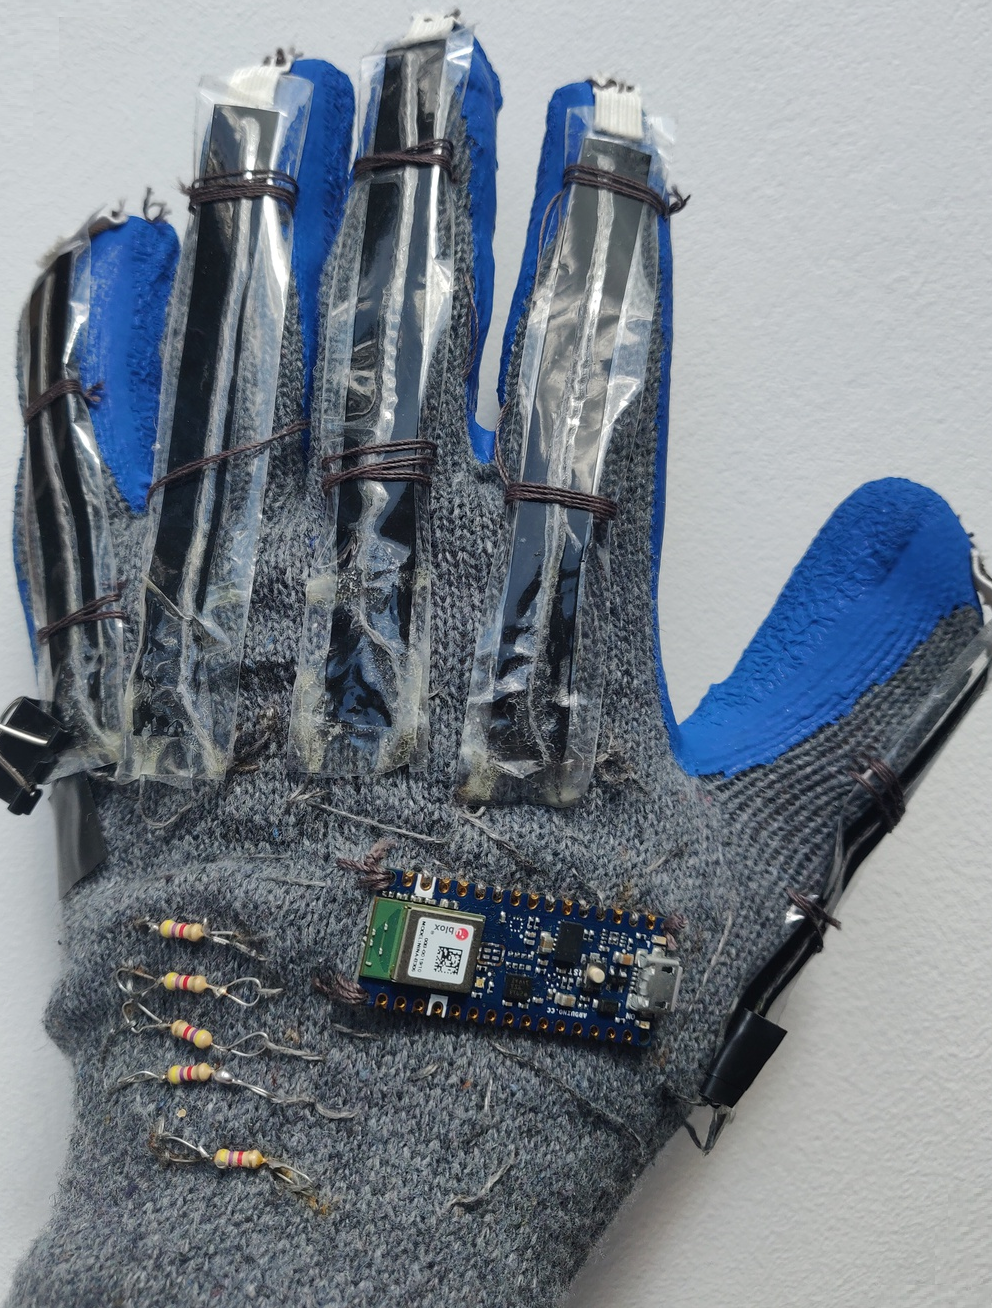
\includegraphics[width=\textwidth]{glove}
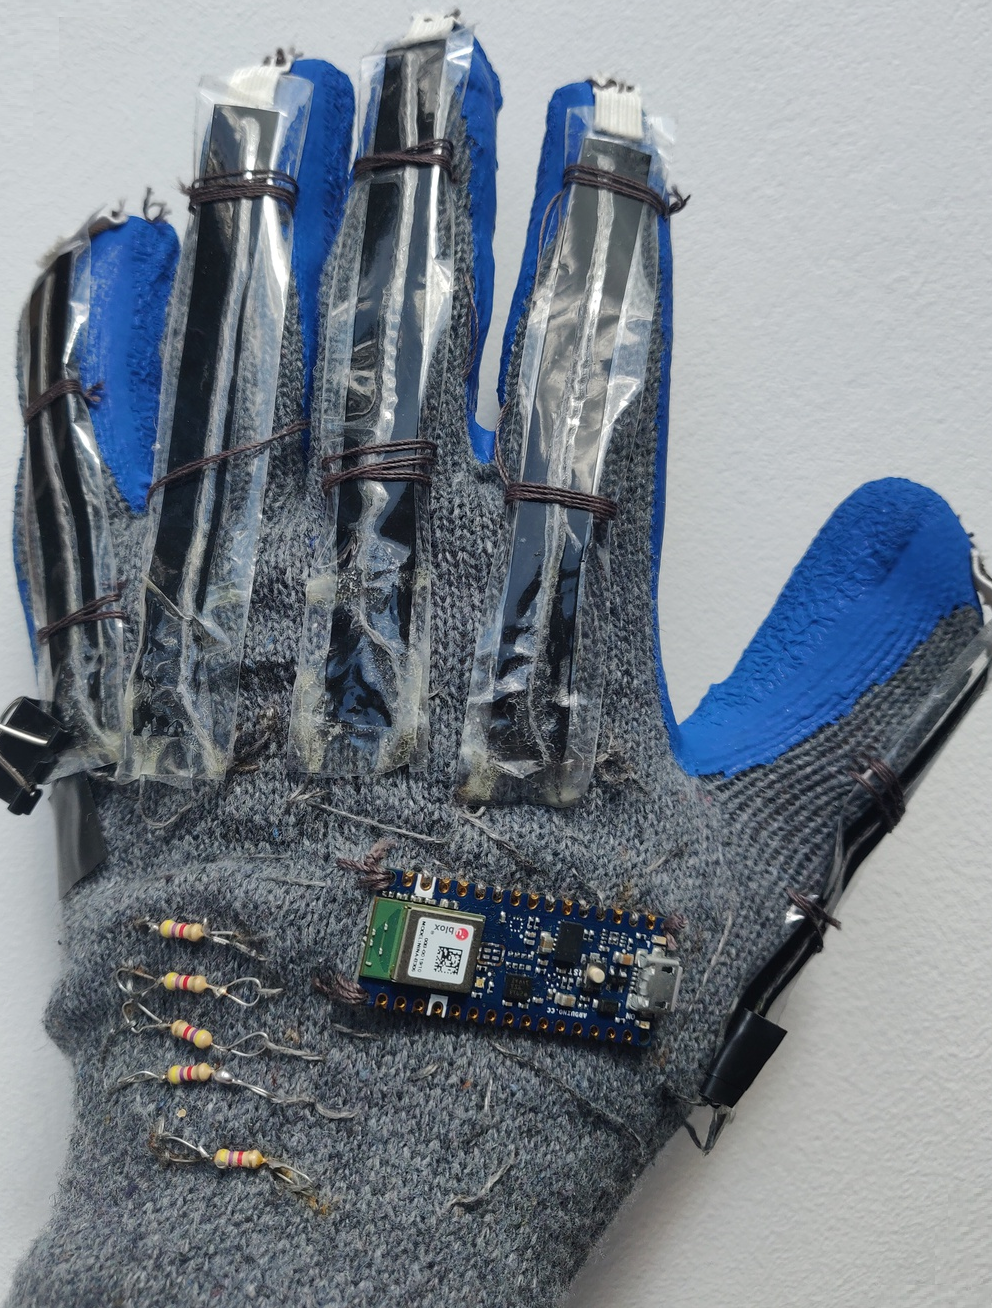
\includegraphics[scale = 0.35]{glove}
\caption{Efekt końcowy rękawicy-kontrolera}
\label{fig:glove}
\end{figure}

\section{Oprogramowanie mikrokontrolera}
\label{sec:oprogramowanie}


Do tej pory została opisana teoria omawianego kontrolera, elementy które zostały użyte w projekcie a także sposób ich połączenia. W niniejszej sekcji przedstawiony jest kod programu który został napisany w środowisku programistycznym oraz języku o tej samej nazwie - Arduino. Język ten poza drobnymi zmianami opiera się na języku C/C++, a jego pełny kod źródłowy jest dostępny na platformie Github~\cite{jArduino}. Aby rozpocząć pracę z wybranym produktem od Arduino należy wykonać pewne czynności przygotowywacze, takie jak instalacja sterowników płytki dla danego systemu czy sposób obsługi w samym środowisku Arduino. Czynności te zostały opisane na stronie producenta, w związku z czym nie zostaną one szczegółowo opisane~\cite{guideArduino}. Po spełnieniu wszystkich wymagań, został przygotowany program który został napisany oraz wgrany do mikrokontrolera, który można podzielić na trzy części:
\begin{itemize}
\item Deklaracje
\item Ustawienie mikrokotrnolera
\item Główna pętla programu
\end{itemize}
których cel oraz opis został przedstawiony poniżej.

W pierwszej kolejności zostanie przedstawiona część deklaracji, w której to dołączono wymagane biblioteki dla poprawnej obsługi wszystkich sensorów. Pierwszą biblioteką która została dołączona do programu jest \textit{Arduino\textunderscore LSM9DS1.h}. Biblioteka ta jest odpowiedzialna za obsługę IMU która przekazuje dane poprzez I2C do mikroprocesora. Biblioteka ta zajmuję się obsługą połączenia jak i kalibracja całego modułu. Inicjalizacja wartości poprzez biblitoekę wygląda w następujący sposób~\cite{ArduinoIMU}
\begin{center}
\begin{tabular}{|c|c|c|}
\hline
Sensor & Zakres & Częstotliwość \\ \hline
Akcelerometr & $[-4,+4]g -/+0.122 mg$ & $104 Hz$\\ \hline
Żyroskop & $[-2000, +2000] dps +/-70 mdps$ & $104 Hz$\\ \hline
Magnetometr & $[-400, +400] uT +/-0.014 uT$ & $20 Hz$ \\ \hline
\hline
\end{tabular}
\end{center}
Tak jak wspomniano w sekcji~\ref{subsec:arduino} do połączenia bezprzewodowego Arduino Nano 33 BLE wykorzystuje moduł Bluetooth Low Energy, w związku z czym w części deklaracji dołączamy przeznaczoną do tego bibliotekę o nazwie \textit{ArduinoBLE.h}. Biblioteka ta pozwala na dostęp oraz sterowanie modułem BLE ( z ang. Bluetooth Low Energy), i na potrzeby projektu zostaną opisane używane elementy z poniższych klasy których znajomość jest wymagana w celu zrozumienia napisanego programu. Klasy te to
\begin{itemize}
\item BLEService
\item BLECharacteristic
\item BLEDescriptor
\item BLE
\item BLEDevice
\end{itemize}
Szczegóły na temat zasad działania BLE są podane w sekcji~\ref{sec:bvsble}, w tej sekcji jedynie zostanie opisana struktura tych klas. \textit{BLEService} umożliwia nawiązanie połączenia z innym urządzeniem obsługującym bluetooth i jako parametr przyjmuje UUID - jest to jedyny paramater jaki należy podać i w ten sposób zostaje stworzony nowy serwis BLE dostępny pod tym identyfikatorem. Klasa \textit{BLECharacteristic} tworzy nową cechę którą należy przypisać do danego serwisu. Cecha ta może zostać zadeklarowana jako cecha wybranego z pośród dostępnych typów w Arduino bądź jako uniwersalna poprzez podstawową klasę \textit{BLECharacteristic}. Klasa ta przyjmuje trzy wymagane parametry: UUID, właściwości cechy oraz wartość. Wartość może zostać zadeklarowana jako podany ciąg znaków, bądź też poprzez określenie rozmiaru danych i wartość początkową. Wartość początkowa nie musi być podana w trakcie deklaracji. Ważnym elementem tej klasy jest określenie jej właściwości. W zależności od przeznaczenia mamy do wybory następujące opcje, które mogą być ze sobą łączone: BLEBroadcast, BLERead, BLEWriteWithoutResponse, BLEWrite, BLENotify, BLEIndicate. W celu wysyłania danych podczas gdy dane te się zmienią cechy w prezentowanym programie przyjęły dwie wartości BLE: read ( z ang. czytać) oraz notify (z ang. powiadomić). Klasa \textit{BLEDescriptor} jest niejako klasą pomocniczną. Wartości tej klasy przypisuję się do danej cechy w celu lepszej obsługi serwisy oraz łatwiejszego rozpoznawania w przypadku pracy ze skomplikowanymi serwisami. Standardowo należy podać UUID danego deskryptora jako parametr, a także jego wartość jako ciąg znaków, bądź wartość w postaci tablicy bajtów oraz maksymalnego rozmiaru danych. Są to podstawowe klasy znajdujące się w części deklaracji których użycie zostały przedstawione na listingu~\ref{lst:declaration} prezentującym wycinek części deklaracji~\cite{ArduinoBLE}. Pozostałe dwie klasy zostaną opisane w części głównej pętli programu gdzie zostanie również pokazane ich zastosowanie. 

\begin{lstlisting}[caption={Część deklaracji programu mikrokontrolera},captionpos=b,label={lst:declaration},language = C++ , frame = trBL , firstnumber = last , escapeinside={(*@}{@*)}]
#include <Arduino_LSM9DS1.h>
#include <ArduinoBLE.h>
BLEService imuService("1101");

BLECharacteristic imuAccChar("2101", BLERead | BLENotify,12);
BLECharacteristic imuGyroChar("2102", BLERead | BLENotify, 12);
BLECharacteristic fingersChar("2103", BLERead | BLENotify, 20);

BLEDescriptor     imuAccDescriptor("3101",(byte*)"Acc Descriptor",15);
BLEDescriptor     imuGyroDescriptor("3102",(byte*)"Gyr Descriptor",15);
BLEDescriptor     fingersDescriptor("3103",(byte*)"Fin Descriptor",15);
\end{lstlisting}

Następną częścią programu jest ustawienie mikrokontrolera oraz sprawdzenia poprawności działania sensorów. Gdy proces ten zakończy się powodzeniem zostanie uruchomiona główna część programu - funkcja \textit{loop()}, która wykonuję się nieprzerwania pozwalając kontrolować pracę naszego kontrolera. Za część związaną z inicjalizacją jest odpowiedzialna funkcja \textit{setup()}. Funkcja ta jest wywoływana tylko raz za każdym razem gdy płytka jest podłączona do prądu bądź zostanie zresetowana~\cite{ArduinoDoc}. W funkcji tej wywoływana jest statyczna metoda begin(z ang. rozpocząć) na klasie \textit{IMU} która należy do biblioteki \textit{Arduino\textunderscore LSM9DS1.h}, i to właśnie ta funkcja pozwala na incjalizacje wspominanych sensorów wchodzących w skład jednostki pomiarowej - program zapętli się w tym miejscu jeśli funkcja ta zwróci błąd, poprzez rozpoczęcie pętli z warunkiem zawsze prawdziwym, co przedstawia listing~\ref{lst:init}~\cite{ArduinoIMU}. 
\begin{lstlisting}[caption={Inicjalizacja IMU oraz BLE},captionpos=b,label={lst:init},language = C++ , frame = trBL , firstnumber = last , escapeinside={(*@}{@*)}]
  if (!IMU.begin()) {
    Serial.println("Failed to initialize IMU!");
    while (1);
  }

  if (!BLE.begin()) {
    Serial.println("Failed to start Bluetooth!");
    while (1);
  }
\end{lstlisting}
Jeżeli sensory działają poprawnie, sprawdzana jest możliwość połączenia poprzez moduł bezprzewodowy. W tym celu wykorzystywana jest statyczna klasa \textit{BLE}, która odpowiada za włączenie modułu Bluetooth oraz jego ustawienia. Tak jak w przypadku klasy \textit{IMU}, program zapętli się w tym miejscu zwracając błąd jeżeli połączenie nie będzie możliwe. W przypadku powodzenia program rozpoczyna łączenie zadeklarowanych elementów, takich jak serwis, cechy oraz deskryptory tych cech. Klasa \textit{BLE} posiada funkcje pozwalającą ustawić nazwę dla naszego połączenia, jej adres a przede wszystkim gdy wszystkie elementy są już gotowe wywołuję metodę \textit{advertise()}, która pozwala na połączenie się z naszym serwisem. Na listingu~\ref{lst:initBle} pokazane jest szczegółowa konfiguracja klasy BLE oraz serwisu a także odpowiednie użycie funkcji dla jednej z cech, które należy powtórzyć dla każdej dodawanej cechy z odpowiednimi wartościami.
\begin{lstlisting}[caption={Obsługa serwisu przy użycia klasy BLE},captionpos=b,label={lst:initBle},language = C++ , frame = trBL , firstnumber = last , escapeinside={(*@}{@*)}]
  BLE.setLocalName("VrGlove");  
  BLE.setAdvertisedService(imuService);

  imuService.addCharacteristic(imuGyroChar);
  imuGyroChar.addDescriptor(imuGyroDescriptor);
  imuGyroChar.writeValue((byte)0x01);
  
  BLE.addService(imuService);     
  BLE.advertise();
\end{lstlisting}
W ten oto sposób kończy się funkcja \textit{setup()} i zostaje wywołana kolejna funkcja która od tej pory będzie odpowiedzialna za pracę kontrolera - \textit{loop()}. W funkcji tej zostaje zadeklarowana ostatnia z wymienionych klas do obsługi Bluetooth. Klasa ta nazywa się \textit{BLEDevice} i jest bezpośrednio powiązana z urządzeniem które jest aktualnie podłączone. Dopóki nie ma podłączonego do kontrolera urządzenia, żadne czynności nie zostają podjęte. W momencie uzyskania danych z modułu łączności o nawiązanym połączeniu zostaje uruchomiona pętla, funkcjonująca tak długo jak połączenie to nie zostanie przerwane. Fragment kodu znajduję się na listingu~\ref{lst:central}~\cite{ArduinoBLE}. Niestety w trakcie pracy z urządzeniem odkryto błąd związany z rozłączeniem się centrali. Problem pojawia się gdy urządzenie zostaję rozłączone z mikrokontrolerem - w tym momencie klasa \textit{BLE} nie zawsze zgłasza informację o rozłączeniu, myśląc że urządzenia cały czas są podłączone. Problem został zauważony, jednak nie jest rozwiązany na stan z maja 2020 roku~\cite{ArduinoBug}. 
\begin{lstlisting}[caption={Oczekiwanie na połączenie z urządzeniem przez mikrokontroler},captionpos=b,label={lst:central},language = C++ , frame = trBL , firstnumber = last , escapeinside={(*@}{@*)}]
  BLEDevice central = BLE.central();
  if (central) {
    Serial.print("Connected to central: ");
    Serial.println(central.address());
  }  
   while( central.connected()){ 
   		[...]
   	}
\end{lstlisting}
Gdy wszystkie dotychczasowo opisane elementy programu nie zgłoszą problemów, następuje ostatnia faza którą jest zbieranie i przesyłanie danych. W pierwszej kolejności sprawdzany jest warunek czy jednostka pomiarowa ma dostęp do nowych danych. W przypadku tej aplikacji dane które zostały poddane analizie pochodzą z żyroskopu oraz z akcelerometru i są wyrażone jako zmienne x,y oraz z typu \textit{float}. Z powodu naturalnych drgań dłoni dane te ciągle się zmieniają w mikro skali która nie ma wpływu na efekty, niemniej jednak możemy założyć że gdy mikroprocesor nie jest przymocowany do stałego obiektu, dane te będą dostarczane z częstotliwością pracy sensorów. Za odczyt danych z żyroskopu i akcelerometru odpowiadają odpowiednio funkcje \textit{readGyroscope(x,y,z)} oraz \textit{readAcceleration(x,y,z)} z klasy \textit{IMU} które przypisuję odpowiednie wartości do podanych parametrów. Ważnym elementem podczas odczytu tych danych jest tak zwany szum który powstaje w trakcie przygotowania sensorów. W trakcie pierwszych odczytów szum ten został zmierzony oraz usunięty z pomiarów. Akcelerometr położony na płaskim obiekcie prawidłowo podawał odczyty, czyli zwracał wektor $[0,0,g]$ gdzie \textit{g} oznacza grawitacje ziemską. Żyroskop natomiast wskazywał błąd rzędu $[2.80,0.18,0.18]$ w związku  z czym od każdego odczytu właśnie taką wartość należy odjąć w celu uzyskania prawidłowych danych - czyli wektora zbliżonego do $[0,0,0]$ w pozycji w której został skalibrowany. Jak wspomniano w sekcji~\ref{subsec:gyro} dotyczącej żyroskopu, wartości zwracane są podane w $dps$ (z ang. Degrees per second) czyli w kątach na sekundę. W celu określenie kątów w jakim urządzenie się znajduję w danym momencie musimy te dane przemnożyć przez częstotliwość z jaką są one pobierane - czyli przemnożyć przez czas co zwróci nam miarę kątów. Osiągamy to poprzez zapisanie czasu w którym dane zostały pobrane a także poprzez zapisanie tej wartości przed następnym pobraniem danych jako czas ostatniego poboru. Różnica pomiędzy tymi wartościami daje czas jaki upłynął aby uzyskać nowe wartości. Zaczynając w pozycji kalibracyjnej, z idealnie usuniętym szumem, żyroskop zwróci wartość zero, a wraz ze zmianą wartości żyroskopu, suma tych zmian wskaże na orientację kontrolera względem pozycji wyjściowej. Więcej informacji na ten temat znajduję się w rozdziale~\ref{ch:aplikacja}~\cite[gimbal]. Ostatnią cechą którą chcemy przekazać są dane pobierane z sensorów wygięcia w celu określenia pozycji palców. Tak jak wspomniano w sekcji~\ref{sec:przeglad} dane te pobieramy przez mierzenie napięcia jakie znajduje się na poszczególny analogowych pinach wejściowych. Odczyty te uzyskujemy poprzez wywołanie metody \textit{analogRead(pin)}~\cite{ArduinoDoc}. Pobieranie danych oraz ich wstępna obróbka przedstawia listing~\ref{lst:read}.
\begin{lstlisting}[caption={Wczytywanie danych z sensorów.},captionpos=b,label={lst:read},language = C++ , frame = trBL , firstnumber = last , escapeinside={(*@}{@*)}]
 if (IMU.accelerationAvailable() && IMU.gyroscopeAvailable()) {
        previousTime = currentTime;
        currentTime = millis();
        elapsedTime = (currentTime - previousTime) / 1000;   

        IMU.readAcceleration(acc[0],acc[1], acc[2]);  
        IMU.readGyroscope(gyro[0],gyro[1], gyro[2]);
        
        gyro[0] -= 2.80;
        gyro[1] -= 0.18;
        gyro[2] -= 0.18;

        fingers[0] = analogRead(A3);
        [...]
 }
\end{lstlisting}
Na tym etapie mamy już dostęp do danych z akcelerometru w {\Large $\frac{m}{s^2}$} oraz dane z żyroskopu wyrażone w stopniach. Informacje te mogłyby zostać przesłane w takiej formie, jednak z racji znajomości projektu, dane można dodatkowo skorygować poprzez zastosowanie dodatkowych filtrów. Podstawowym zabiegiem który został zastosowany jest eliminacja danych nieznaczących, czyli szumu który powstaje poprzez naturalne drgania ciała. Aby to osiągnąć, w programie przechowywane są poprzednie wartości z poszczególnych sensorów. Jak dane znaczące dla akcelerometru przyjęto różnice $\pm 0.1$, a dla danych z sensorów wygięcia $\pm 15$. Dla żyroskopu natomiast przyjęto wartości różniące się o przynajmniej $\pm 0.2$, a także dodatkowo sprawdzane jest czy dane z żyroskopu nie są w pozycji przy kalibracyjnej. Oznacza to że jeżeli wartości zwracane z żyroskopu wynoszą $0\pm 0.1$, zostaną one zamienione na wartość równą $0$. Filtrowanie wartości pokazane jest na listingu~\ref{lst:filtr}. W ten oto sposób otrzymano wartości z sensorów które były gotowe do wysłania na inne urządzenie. Wartości te jednak są wyrażone w postaci tablic typu \textit{float}, natomiast jako wartości cechy bluetooth przyjmują tablice bytów. W związku z tym przed przypisaniem danych są przekazywane adresy tablic do nowych zmiennych, a następnie zmienne te zapisane w poszczególnej cesze przy użyciu metody \textit{setValue(value,valueSize)}. Rozmiar jest ten określony jako $12$ ponieważ mamy do czynienia z tablicą 3 zmiennych typu \textit{float} z których każda zajmuje 4 bajty pamięci. Zapisywanie danych jest pokazana na listingu~\ref{lst:save} dla jednej cechy - proces ten należy powtórzyć dla wszystkich danych. Program następnie zapisuje obecne dane jako dane obecnej pętli, tak aby następne odczyty mogły zostać porównane z obecną iteracją, tym samym kończąc wykonywaną pętle. Warto zauważyć że program pomimo swojego głównego działa w funkcji \textit{loop()}, jest wykonywany w ramach jednej iteracji jak tylko dojdzie do połączenia kontrolera z odbiornikiem.
\begin{lstlisting}[caption={Wstępne filtrowanie danych z sensorów.},captionpos=b,label={lst:filtr},language = C++ , frame = trBL , firstnumber = last , escapeinside={(*@}{@*)}]
for (int i = 0;i<3;i++){
	if(!(gyro[i] < oldGyroData[i]-0.2 || gyro[i] > oldGyroData[i]+0.2)){
		if( gyro[i] < -0.1 ||  gyro[i] > 0.1){              
	      gyro[i] = oldGyroData[i];
	    }else{
	     gyro[i] = 0.0;
	    }
	}
	            
	if(!(acc[i] < oldAccData[i]-0.02 || acc[i] > oldAccData[i]+0.02)){
	   acc[i] = oldAccData[i];
	   }
}

for (int i = 0;i<5;i++){
   if(!(fingers[i] < oldFingersData[i]-15.0 || fingers[i] > oldFingersData[i]+15.0)){
              fingers[i] = oldFingersData[i];
            }
         }         
 }
\end{lstlisting}

\begin{lstlisting}[caption={Zapisywanie danych do cech w serwisie.},captionpos=b,label={lst:save},language = C++ , frame = trBL , firstnumber = last , escapeinside={(*@}{@*)}]
         byte *accChar = (byte*)&acc;
         imuAccChar.setValue(accChar,12);
\end{lstlisting}

\section{Podsumowanie}
\label{sec:summary}
W tym rozdziale podano informacje na temat projektu rękawicy kontrolera a także elementów które są wymagane w celu jego funkcjonowania. Zostały podane specyfikacje podzespołów, sposoby pozyskiwania danych, metoda komunikacji z innymi urządzeniami a także rozwiązano problemy związane z kosztem projektu. Krok po kroku przedstawiono złożenie elementów w celu uzyskania końcowej wersji produktu i ostatecznie omówiono zasadę działania programu napisanego w Arduino wraz z bibliotekami które zostały użyte w ramach projektu, natomiast zasady ich praktycznego działania zostały pokazane na listingach. W ten oto sposób została zakończona główna część projektu, pozwalająca na wykorzystanie rękawicy kontrolera jako część większych przedsięwzięć. Aby jeszcze lepiej zobrazować sposób obsługi kontrolera, oraz metody wykorzystania danych, w rozdziale~\ref{ch:aplikacja} zostanie pokazana przykładowa aplikacja wykorzystująca dane w celu analizy oraz prezentacji. 
\chapter{Dedykowana aplikacja w systemie Android}
\label{ch:aplikacja}
W tym rozdziale pokazana zostanie przykładowa aplikacja która współpracuję z rękawicą-kontrolerem. Aplikacja ta ma za zadanie wyświetlanie aktualnego stanu sensorów rękawicy oraz połączenia, a także prezentowanie tych danych. Pomimo możliwości wykorzystania wielu dostępnych platform do tworzenia animacji oraz środowisk wirtualnych, zdecydowano się na napisanie aplikacji na system Android wykorzystując do tego język Java. Aplikacja ta pozwala na wysoką mobilność, zagłębienie się w tematykę BLE, dzięki zaprogramowaniu własnego połączenia z serwisem udostępnianym przez rękawicę, a także łatwe zaznajomienie się z działaniem rękawicy nawet bez żadnej informacji dotyczącej jej obsługi. Rozdział ten przedstawia interfejs użytkownika, sposób komunikacji z rękawicą-kontrolerem a także opis używanego przez aplikację SDK o nazwie \textit{Google Sceneform}. Dołączony projekt firmy Google pozwala na importowanie modeli dłoni do aplikacji, prezentację ich a także odpowiada za animację na ekranie. W tym rozdziale zostaną pokazane zaimplementowane rozwiązania z którymi mierzą się twórcy kontrolerów, w szczególności przy wykorzystaniu nawigacji inercyjnej.

\section{Interfejs użytkownika}
\label{sec:interface}
W niniejszej sekcji opisano interfejs wraz z jego elementami oraz ich funkcjonalność w ramach całej aplikacji. Aplikacja składa się z jednej aktywności o nazwie \textit{MainActivity} w ramach której został zaimplementowany układ zakładek, a konkretnie dwóch zakładek - dane oraz animacja. Zakładki te odpowiednio są uzupełnianie przygotowanymi fragmentami poprzez klasę \textit{SectionsPagerAdapter} oraz \textit{ViewPager}.W celu odpowiedniej obsługi fragmentów, aktywność ta musi implementować metody interfejsu \textit{OnFragmentInteractionListener}, które są zadeklarowane w klasach \textit{ModelRenderer} oraz \textit{GloveData}. Klasy te aby spełnić swoją funkcjonalność dziedziczą po klasie \textit{Fragment}~\cite{AndroidDoc}. W ten oto sposób zadeklarowano trzy klasy na podstawie których wyświetlany jest interfejs użytkownika, przedstawiony na rysunku~\ref{fig:ifce}. Metodę \textit{onCreate(Bundle)} przedstawia lsiting~\ref{lst:crt} na którym to widać krok po kroku sposób ładowania fragmentów w aktywności.
\begin{lstlisting}[caption={Interfejs użytkownika.},captionpos=b,label={lst:crt},language = Java , frame = trBL , firstnumber = last , escapeinside={(*@}{@*)}]
    @Override
    protected void onCreate(Bundle savedInstanceState) {
        super.onCreate(savedInstanceState);
        setContentView(R.layout.activity_main);
        SectionsPagerAdapter sectionsPagerAdapter = new SectionsPagerAdapter(this, getSupportFragmentManager());
        ViewPager viewPager = findViewById(R.id.view_pager);
        viewPager.setAdapter(sectionsPagerAdapter);
        TabLayout tabs = findViewById(R.id.tabs);
        tabs.setupWithViewPager(viewPager);

        IntentFilter filter = new IntentFilter(BluetoothAdapter.ACTION_STATE_CHANGED);
        registerReceiver(mReceiver, filter);
    }
\end{lstlisting}
Dwie ostatnie linie listingu pokazują wywołanie rejestracji odbiornika w celu otrzymywania informacji dotyczącego modułu Bluetooth wbudowanego w urządzenia na którym aplikacja jest uruchomiona. Oprócz wspominanych do tej pory klas, aplikacja korzysta również z dodatkowej klasy o nazwie \textit{VrGlove}, służącej do przechowywania informacji na temat kontrolera. Więcej informacji o tej klasie oraz o odbiorniku modułu Bluetooth zostanie przedstawionych w sekcji~\ref{sec:komunikacja}. 

\begin{figure}[h]
\centering
	\begin{subfigure}[b]{0.45\textwidth}
	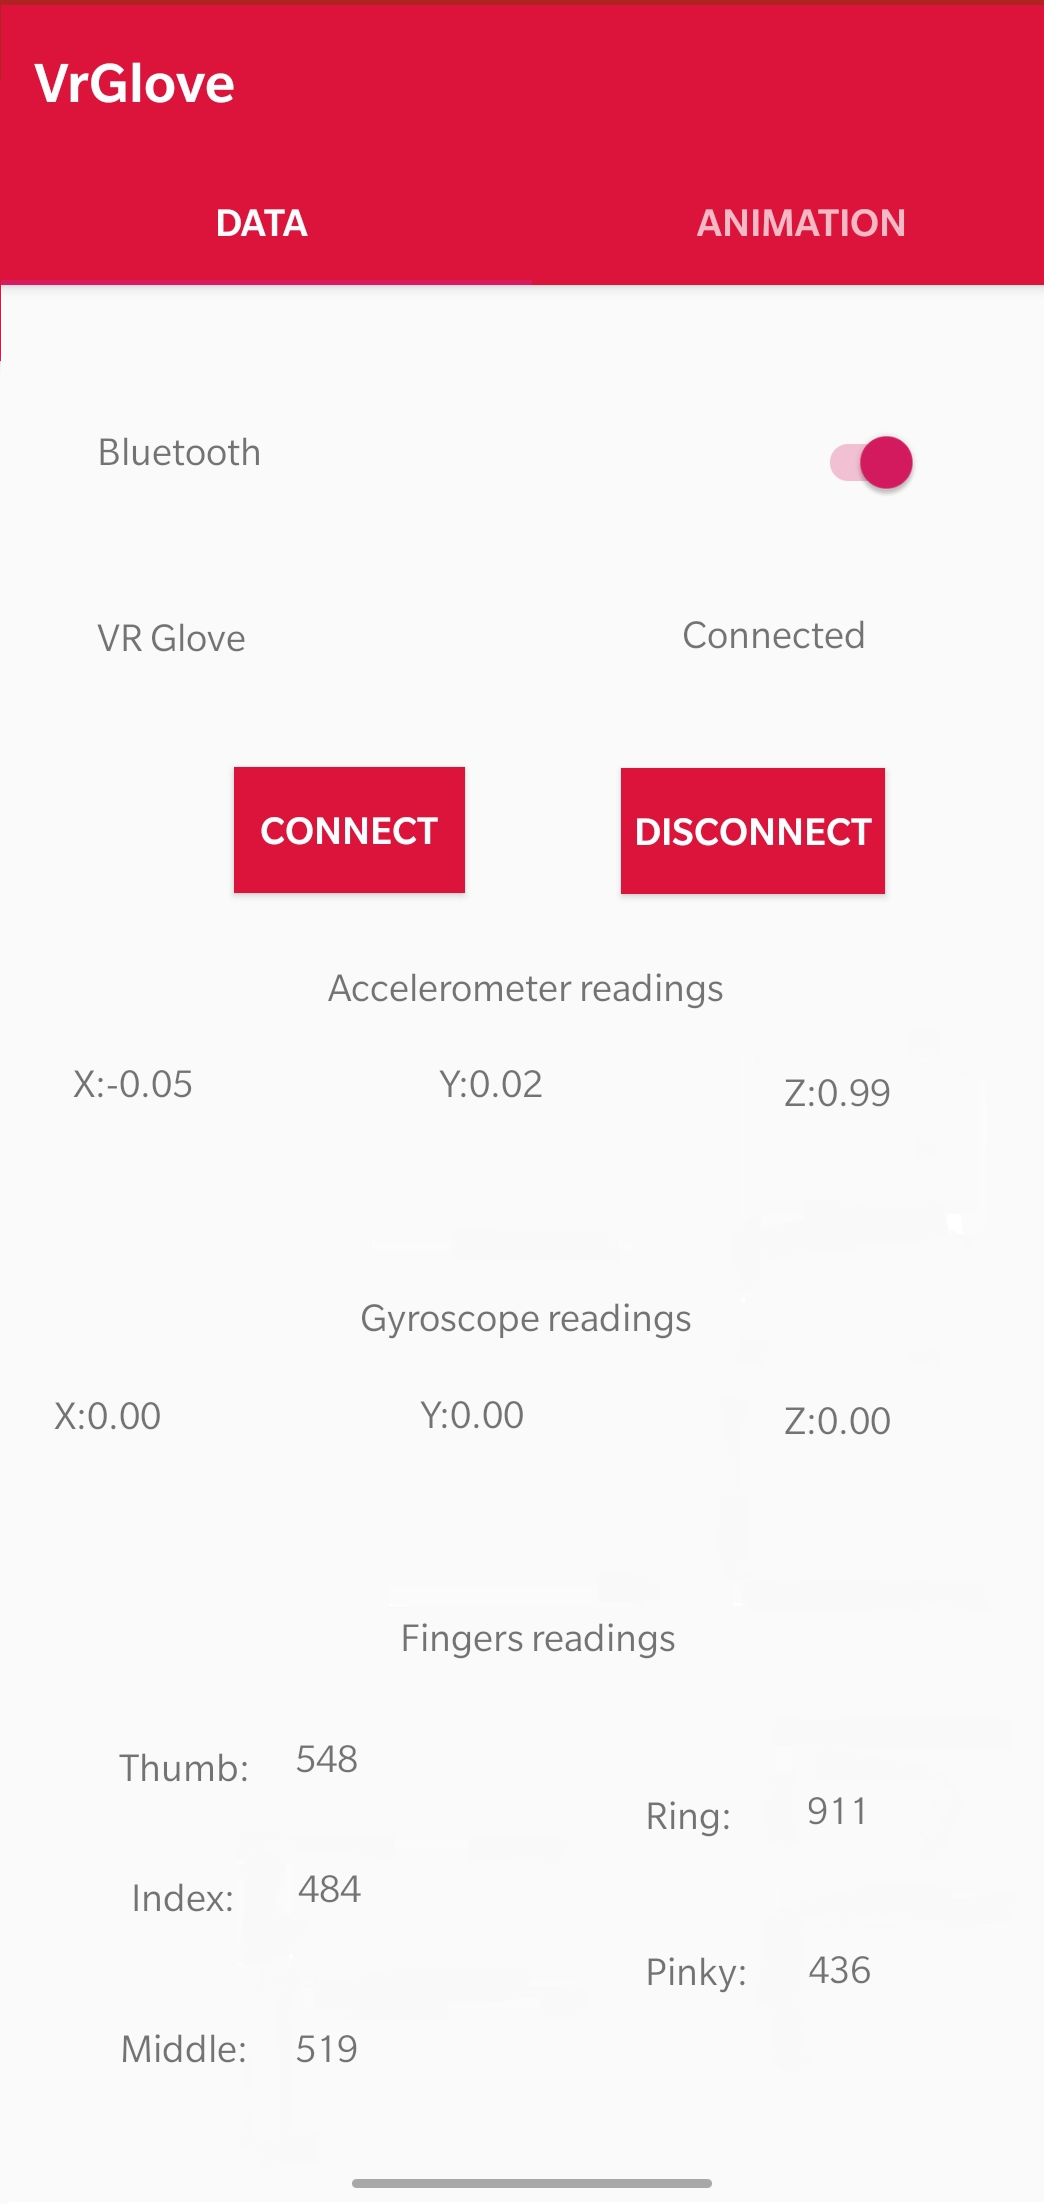
\includegraphics[width=\textwidth]{UI1}
	\caption{Fragment prezentujący dane}
	\label{fig:ifceDane}
	\end{subfigure}
	~
	\begin{subfigure}[b]{0.45\textwidth}
	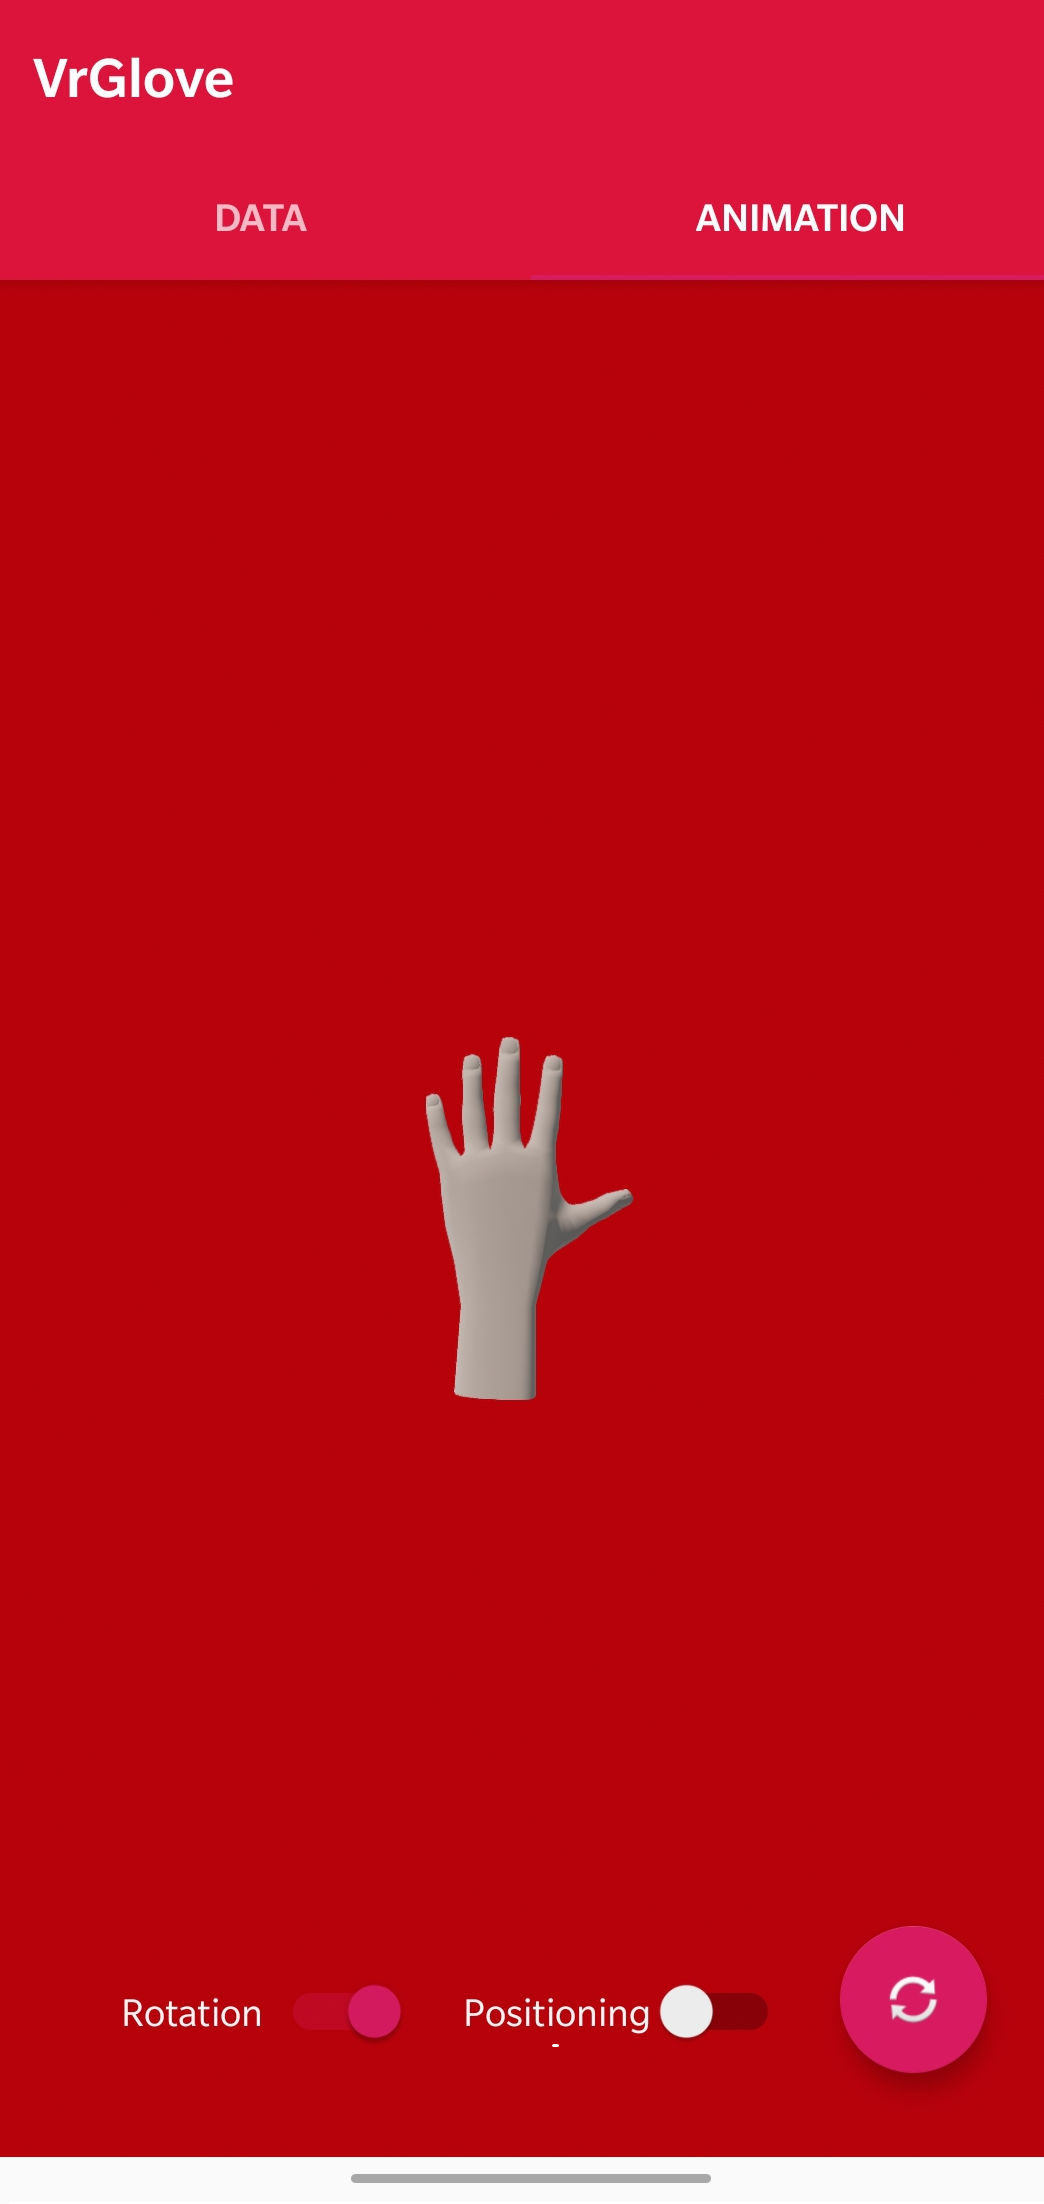
\includegraphics[width=\textwidth]{UI2}
	\caption{Fragment prezentujący animacje}
	\label{fig:ifceAnimacja}
	\end{subfigure}
\caption{Interfejs użytkownika}
\label{fig:ifce}
\end{figure}

Jak widać na~\ref{fig:ifceDane} rozpoczynając od góry widzimy informację dotyczącą obecnego stanu modułu Bluetooth w urządzeniu, wyrażanego poprzez przycisk przełącznika, pozwalający na włączenie/wyłączenie modułu bezpośrednio z poziomu aplikacji. Pod spodem Widnieje informacja o możliwości połączenia/statusie połączenia z kontrolerem opisana etykietą VR Glove. Etykieta ta przyjmuje następujące wartości:
\begin{itemize}
\item Włącz Bluetooth (ang. Turn On Bluetooth)
\item W trakcie włączania (ang. Turning On)
\item W trakcie wyłączania (ang. Turning Off)
\item Gotowy do połączenia (ang. Ready to connect)
\item W trakcie łączenia (ang. Connecting)
\item Połączony (ang. Connected)
\item W trakcie rozłączania (ang. Disconnecting)
\item Rozłączony (ang. Disconnected)
\end{itemize}
\label{itm:stany}
Pierwsze trzy stany możemy osiągnąć poprzez włączanie/wyłączanie modułu Bluetooth w urządzeniu. Stan gotowości do połączenia pokazuję się gdy moduł bluetooth został włączony i jest gotowy do połączenia z kontrolerem. Dwa przyciski znajdujące się poniżej etykiety, odpowiednio \textit{połącz (ang. Connect)} i \textit{rozłącz (ang. Disconnect)} pozwalają na połączenie z rękawicą-kontrolerem. Ostatnie cztery stany obrazują status połączenia z rękawicą, który możemy zmienić korzystając odpowiednio z przycisków. Poniżej znajdują się etykiety dotyczące sensorów kontrolera które są puste gdy aplikacja nie została jeszcze połączona z kontrolerem. Pola ta odpowiednio od góry reprezentują wartości zwracane przez akcelerometr i żyroskop jako wartości X,Y i Z, oraz wartości sensorów znajdujących się na palcach, z każdym sensorem mającym własną etykietę. Drugą częścią interfejsu prezentuje~\ref{fig:ifceAnimacja}, na której to widoczna jest lewa dłoń, znajdujące się na środku ekranu. Pozycja ta jest przyjmowana zanim kontroler zostanie podłączony. W dolnej części ekranu widzimy dwa przyciski przełączniki, służące do regulowania modelu, pozwalając decydować nam które elementy mają być brane pod uwagę podczas generowania animacji. Od lewej odpowiednio możliwe jest do zmiany branie pod uwagę orientacji kontrolera przy generowaniu modelu, następnie jego pozycji względem pozycji kalibracyjnej, oraz ostatni element tego interfejsu czyli FAB(ang. Floating Action Button) - służący do ponownej kalibracji dłoni. Kalibracja ta jest również wywoływana przy każdej zmianie decyzji dotyczącej generowania rotacji bądź położenia. Pozycją kalibracyjną jest pozycja w której lewa dłoń na której znajduje się rękawica-kontroler, wraz ze wszystkimi palcami znajduję się w pozycji wyprostowanej, a kciuk wskazuje ciało użytkownika. Interfejs ten pozwala na szybkie połączenie się z kontrolerem a gdy tylko pierwsze dane zostaną przesłane do aplikacji, natychmiastowo obserwujemy pracę kontrolera na ekranie smart-fona. Warto zauważyć że po włączeniu aplikacji przełącznik orientacji jest włączony natomiast pozycjonowanie dłoni na ekranie wyłączone, w związku z czym animacja wyświetla się na środku ekranu. Do tej pory opisano wygląd i informacje elementów znajdujących się na ekranie, dalsza część tego rozdziału pokaże w jaki sposób wspomniane elementy działają od strony kodu źródłowego.

\section{Komunikacja}
\label{sec:komunikacja}
Opis interfejsu aplikacji pokazuje elementy które są wymagane oraz zaprogramowane w aplikacji. Pokazuje jakie dane są używana oraz w jakim celu wykorzystywane. Żeby jednak skorzystać z tych danych najpierw aplikacja musi zostać połączona z kontrolerem. W sekcji~\ref{subsec:arduino} powiedziano o wykorzystywaniu w tym celu połączenia BLE a o tym jak to jest obsługiwane przez prezentowaną aplikacje zostanie pokazane w części~\ref{subsec:ble}. Aby rozpocząć pracę z BLE przede wszystkim należy się upewnić że moduł Bluetooth w urządzeniu jest dostępny oraz włączony. W celu sprawdzenia dostępności modułu bluetooth w urządzeniu wykorzystywany jest plik \textit{AndroidManifest.xml}, w którym to zdefiniowano dostęp. Wszystkie wymagane pozwolenia pokazuje listing~\ref{lst:pozwolenia}.
	\begin{lstlisting}[caption={Wymagane pozwolenia dla aplikacji.},captionpos=b,label={lst:pozwolenia},language = Java , frame = trBL , firstnumber = last , escapeinside={(*@}{@*)}]
    <uses-permission android:name="android.permission.BLUETOOTH" />
    <uses-permission android:name="android.permission.BLUETOOTH_ADMIN" />
    <uses-permission android:name="android.permission.READ_EXTERNAL_STORAGE" />
    <uses-permission android:name="android.permission.CAMERA" />
\end{lstlisting}
Mając wymagany dostęp możemy sterować sensorem poprzez przycisk przełącznika. W kodzie programu wystarczy uzyskać do niego dostęp używając metody \textit{findViewById(int)} a następnie ustawić nasłuchiwacza kliknięć. Przyciski \textit{Połącz} oraz \textit{Rozłącz} są zdefiniowane w ten sam sposób. Aby wprowadzić zmiany w Bluetooth należy użyć klasy \textit{BluetoothAdapter}. Po pobraniu domyślnego adaptera jesteśmy w stanie określić jego stan. używając metod \textit{enable()} oraz \textit{disable()}. Sposób obsługi adaptera jest pokazany na listingu~\ref{lst:switchBT}. Zmiana ta wywołuję funkcję znajdującą się w klasie \textit{MainActivity} która reaguje na zmiany adaptera oraz ustawia jeden z pierwszych czterech statusów z listy~\ref{itm:stany} dla pola definiującego obecny stan połączenia. Skrócony listing~\ref{lst:status} pokazuje wywołanie tej funkcji dla przykładowego stanu adaptera. Ostatnie cztery stany wypunktowane w~\ref{itm:stany} pochodzą ze zmiany połączenia wywoływane poprzez wspomniane przyciski \textit{Połącz} oraz \textit{Rozłącz} które zostoną opisane w sekcji~\ref{subsec:ble}. \newpage
	\begin{lstlisting}[caption={Obsługa wbudowanego modułu Bluetooth.},captionpos=b,label={lst:switchBT},language = Java , frame = trBL , firstnumber = last , escapeinside={(*@}{@*)}]
switch (v.getId()){
            case R.id.switchBT:
            	Switch switchBT = v.findViewById(R.id.switchBT);
        		BluetoothAdapter mBluetoothAdapter = BluetoothAdapter.getDefaultAdapter();
                if (switchBT.isChecked()){
                    if (!mBluetoothAdapter.isEnabled()) {
                        mBluetoothAdapter.enable();
                    }
                }else{
                    if (mBluetoothAdapter.isEnabled()) {
                        mBluetoothAdapter.disable();
                [...]
}
\end{lstlisting}
\begin{lstlisting}[caption={Zmiana statusu na podstawie adaptera bluetooth.},captionpos=b,label={lst:status},language = Java , frame = trBL , firstnumber = last , escapeinside={(*@}{@*)}]
private final BroadcastReceiver mReceiver = new BroadcastReceiver() {
        @Override
        public void onReceive(Context context, Intent intent) {
            final String action = intent.getAction();
            Switch tbBT= findViewById(R.id.switchBT);
            TextView tvStatus = findViewById(R.id.textView_vrGlove_status);
            if (action.equals(BluetoothAdapter.ACTION_STATE_CHANGED)) {
                final int state = intent.getIntExtra(BluetoothAdapter.EXTRA_STATE,
                        BluetoothAdapter.ERROR);
                switch (state) {
                    case BluetoothAdapter.STATE_OFF:
                        tbBT.setChecked(false);
                        tvStatus.setText("Turn on bluetooth");
                        break;
                    [...]
}                    
\end{lstlisting}

	\subsection{Obsługa połączenia Bluetooth Low Energy}
	\label{subsec:ble}
	Gdy poznano stan modułu Bluetooth, bez przeszkód można nawiązać połączenie. w tym celu wykorzystano przyciski sterujące połączeniem. Do przechowywania danych o połączeniu wykorzystywana jest klasa \textit{VrGlove}, w której zdefiniowano statyczne zmienne klasy \textit{BluetoothDevice} pozwalające na wybranie odpowiedniego urządzenia z puli dostępnych urządzeń w pobliży poprzez jego adres oraz \textit{BluetoothGatt} odpowiedzialnej za obsługę serwisu GATT w androidzie. Listę dostępnych serwisów otrzymano deklarując zmienną implementującą listę klasy  \textit{BluetoothGattService}. W ten sposób w dowolnym miejscu programu można odwołać się do klasy kontrolera, sprawdzając jego stan a także uzyskać dane o jego udostępnionych serwisach. Na listingu~\ref{lst:disconnect} pokazano dostęp do klasy rękawicy z nasłuchiwacza przycisku \textit{Rozłącz}. Fragment ten sprawdza czy istnieje aktualnie połączony serwis \textit{GATT} oraz czy jest on w stanie \textit{Połączony} wyrażony jako typ \textit{int} - 2. To właśnie na podstawie tego statusu są określane ostatnie cztery stany połączenia z rękawicą z listy~\ref{itm:stany}. Sposób zmiany statusu są bardzo zbliżone do listingu~\ref{lst:status}, różnica polega na wywołaniu odbiornika zmiany statusu połączenia z klasy \textit{BluetoothGattCallback} w przeciwieństwie do \textit{BroadcastReceiver} oraz zostaje wywołana metoda \textit{onConnectionStateChange} zamiast metody \textit{onReceive}. Jeżeli powyższe warunki są spełnione \textit{GATT} zostaje rozłączony~\cite{AndroidDoc}. 
\begin{lstlisting}[caption={Obsługa przycisku rozłącz.},captionpos=b,label={lst:disconnect},language = Java , frame = trBL , firstnumber = last , escapeinside={(*@}{@*)}]
case R.id.buttonDisconnect:
                if(VrGlove.getGatt() != null && VrGlove.getGattState() == 2 ){
                    VrGlove.getGatt().disconnect();
                }
                break;                    
\end{lstlisting}	
Ostatnia część którą opisano jest zarazem najważniejszą. Mowa o obsłudze przycisku \textit{Połącz}. Tak jak w przypadku przycisky \textit{Rozłącz}, najpierw sprawdzany jest status urządzenia, czyli czy adapter jest włączony oraz w przeciwieństwie do sprawdzania czy nasz serwis \textit{GATT} jest połączony, kod przycisku wykona się tylko wtedy gdy nie jest aktualnie nawiązane połączenie. Gdy warunki te są spełnione, zostaje pobrany adapter bluetooth oraz zostaje podjęta próba połączenia z urządzeniem przy użyciu klasy \textit{BluetoothDevice}, która otrzymuje zwracaną wartość metody \textit{getRemoteDevice(String)} wywołaną na adapterze bluetooth. W naszym przypadku jako parametr typu \textit{String}, zostaje podany adres D0:6B:F2:A7:95: 03, który jest adresem rękawicy-kontrolera z którym zostanie podjęta próba połączenia. Następnie zostaje stworzona nowa instancja klasy \textit{VrGlove}, której zostaje przekazana w parametrach wartość zmiennej typu \textit{BluetoothDevice} oraz aktualny widok na którym pracuje fragment. Posiadając te informacje rozpoczyna się kluczowy etap połączenia, mianowicie zostaje zainicjalizowana zmienna klasy \textit{BluetoothLeScanner}, poprzez wywołanie metody \textit{getBluetoothLeScanner()} na adapterze urządzenia. Metoda ta pozwala na wyszukiwanie urządzeń BLE znajdujących się w pobliżu, poprzez wywołanie metody \textit{startScan(ScanCallback)}, gdzie jako parametr zostaje podany stworzony skaner, oczekujący na pojawienie się urządzenia z wcześniej podanym adresem. Bardzo ważnym elementem jest zatrzymanie skanera gdy zostaje odnalezione urządzenie - co można osiągnąć poprzez wywołanie metody \textit{stopScan(ScanCallback)}. W ten oto sposób nawiązano połączenie pomiędzy urządzeniami a rezultat tego połączenie zostaje zapisany w postaci ustawienia serwisu \textit{GATT} w klasie \textit{VrGlove}. Opisane powyżej czynności są przedstawione na listingu~\ref{lst:connect}~\cite{AndroidDoc}. Dzięki temu możemy kontrolować połączenie z kontrolerem z dedykowanej aplikacji. Ostatnim elementem poprawnego funkcjonowania jest przekazywanie danych w czasie rzeczywistym pomiędzy odbiornikiem a nadajnikiem, co zostanie pokazane w sekcji~\ref{subsec:dane}. \newpage
\begin{lstlisting}[caption={Kluczowe elementy przycisku \textit{Połącz} pozwalającego na połączenie z kontrolerem.},captionpos=b,label={lst:connect},language = Java , frame = trBL , firstnumber = last , escapeinside={(*@}{@*)}]
final BluetoothManager bluetoothManager =
                            (BluetoothManager) getActivity().getSystemService(Context.BLUETOOTH_SERVICE);
mBluetoothAdapter = bluetoothManager.getAdapter();
[...]
BluetoothDevice device = mBluetoothAdapter.getRemoteDevice("D0:6B:F2:A7:95:03");
new VrGlove(device,vw);                    
[...]
BluetoothLeScanner scanner = mBluetoothAdapter.getBluetoothLeScanner();
scanner.startScan(scanCallback);
[...]
scanner.stopScan(scanCallback);
gatt = VrGlove.getDevice().connectGatt(getActivity(),false,bluetoothGattCallback, TRANSPORT_LE);
VrGlove.setGatt(gatt);                                                           
\end{lstlisting} 

	\subsection{Pobieranie danych}
	\label{subsec:dane}
	Mając do dyspozycji informacja pozyskane w trakcie połączenia, które są przechowywane jako zmienne statyczne w klasie rękawicy, jesteśmy w stanie pozyskać dane które opisano w rozdziale~\ref{ch:rekawica}. W tym celu, po stronie aplikacji należy sprawdzić czy aktualnie jest nawiązane połączenie, co jak już zostało powiedziane oznacza serwis \textit{GATT} w stanie wyrażanym jako \textit{int = 2}.  Gdy potwierdzono połączenie, z klasy \textit{BluetoothGatt} zostaje wywołana metoda \textit{discoverServices()}, która jest wywoływana dopóki nie zostaną wykryte serwisy. Gdy tak się stanie, rezultat odnalezionych serwisów uzyskiwany jest poprzez metodę serwisu \textit{GATT} \textit{getServices()}. Mając dostęp do serwisów - w opisywanym przypadku wiemy z rozdziału dotyczącego rękawicy-kontrolera że jest to tylko jeden serwis, możemy pobrać cechy używając metody \textit{getCharacteristic(UUID)}, które ten serwis posiada. Cechy te zostały pokazane na listingu~\ref{lst:declaration}, oraz zostały przypisane im skrócone UUID wyrażone jako \textit{int} od $0x2101$ do $0x2103$, odpowiednio jako dane akcelerometru, żyroskopu oraz sensorów umiejscowionych na palcach. Implementacje algorytmu z typu \textit{int} do UUID pokazuje metoda \textit{convertFromInteger(int i)} na listingu~\ref{lst:UUID}~\cite{UUID}. 
	\begin{lstlisting}[caption={Zamiana zmiennej int na UUID.},captionpos=b,label={lst:UUID},language = Java , frame = trBL , firstnumber = last , escapeinside={(*@}{@*)}]
	private UUID convertFromInteger(int i) {
        final long MSB = 0x0000000000001000L;
        final long LSB = 0x800000805f9b34fbL;
        long value = i & 0xFFFFFFFF;
        return new UUID (MSB | (value << 32), LSB);
    }                                                       
\end{lstlisting}
Dla każdej cechy zostaje wywołana metoda \textit{readCharacteristic (BluetoothGattCharacteristic)}, która po sprawdzeniu warunków które są wymagane od każdej z cech dla prezentowanej aplikacji ustawia te cechy w trybie powiadomień - etap ten prezentuje listing~\ref{lst:notify}. Tryb powiadomień dla cechy oznacza że dane zostaną pobrane za każdym razem gdy zajdzie w nich jakaś zmiana. Ostatnią częścią jest pobranie deskryptora danej cechy. W ten sposób oprócz nawiązanego połączenia uzyskano dostęp do serwisów oraz cech reprezentowanych przez urządzenie z którym się połączono. Etap ten zaprezentowano na wycinku kodu~\ref{lst:characteristics}. Ważnym elementem tego procesu jest odczytywanie cech pojedynczo, z racji tego że serwis \textit{GATT} obsługuję połączenie tylko z jedną cechą jednocześnie, co oznacza że gdyby spróbowano pobrać następną cechę, podczas gdy połączenie nie zostało zakończone z poprzednią cechą - połączenie to zostanie nadpisane. Obsługę połączenia z cechą zapewnia nadpisanie metody \textit{onCharacteristicChange(BluetoothGatt, BluetoothGattCharacteristic)} wywoływaną  z klasy \textit{BluetoothGattCallback}. Kod został napisany właśnie w tej metodzie ze względu na tryb w jaki cechy zostały ustawione, czyli tryb powiadomień. Dzięki temu funkcja ta zostaje wywołana za każdym razem gdy obserwowane cechy zostaną w jakiś sposób zmienione. W zależności od rozpoznanej cechy, wywoływana jest metoda zmieniające aktualny zestaw danych w klasie kontrolera, co pokazuje listing~\ref{lst:findChar}.
\begin{lstlisting}[caption={Uzyskanie dostępu do cech serwisu.},captionpos=b,label={lst:characteristics},language = Java , frame = trBL , firstnumber = last , escapeinside={(*@}{@*)}]     
if(VrGlove.getGattState() == 2){
	VrGlove.getGatt().discoverServices();                                                   
	[...]
	VrGlove.setServices(VrGlove.getGatt().getServices());
	for (int i = 0x2101;i<0x2104;i++){
    	mCharacteristic = VrGlove.getServices().get(2).getCharacteristic(convertFromInteger(i));
        readCharacteristic((mCharacteristic));
        BluetoothGattDescriptor descriptor = mCharacteristic.getDescriptor(convertFromInteger(0x2902)); 
        [...]
        VrGlove.getGatt().writeDescriptor(descriptor);
}
\end{lstlisting}

\begin{lstlisting}[caption={Ustawienie cechy w trybie powiadomień.},captionpos=b,label={lst:notify},language = Java , frame = trBL , firstnumber = last , escapeinside={(*@}{@*)}]     
private boolean readCharacteristic(final BluetoothGattCharacteristic characteristic) {  
        if(VrGlove.getGatt() == null) {
            Log.e(TAG, "ERROR: Gatt is 'null', ignoring read request");
            return false;
        }
        if(characteristic == null) {
            Log.e(TAG, "ERROR: Characteristic is 'null', ignoring read request");
            return false;
        }
        if((characteristic.getProperties() & PROPERTY_READ) == 0 ) {
            Log.e(TAG, "ERROR: Characteristic cannot be read");
            return false;
        }
        VrGlove.getGatt().setCharacteristicNotification(characteristic, true);
        return true;
    }                                                      
\end{lstlisting}
Następnie funkcje klasy \textit{VrGlove} przypisują zmiennym odpowiadającym sensorom nowe dane oraz dokonują ich konwersji z tablicy typu \textit{byte} do typu \textit{float}.Dane te po obróbce są przypisywane odpowiednim polom w interfejsie użytkownika. Pobieranie danych polega na wycinaniu z tablicy informacji kolejnych 4 bajtów, co jest równoznaczne jednej zmiennej typu \textit{float}. Ważne dla konwersji jest również sposób w jaki dane zostają zamienione - w tym przypadku używana jest notacja \textit{LITTLE\_ENDIAN}. Wykonane kroki pokazuje listing~\ref{lst:setChar} dla odczytu pierwszej wartości z tablicy danych żyroskopu. Proces ten należy wykonać dla wszystkich wartości w danej cesze oraz odpowiednio dla każdej z pobieranych cech~\cite{AndroidDoc}.
\begin{lstlisting}[caption={Przypisywanie danych pozyskanych z cech, do zmiennych w aplikacji.},captionpos=b,label={lst:setChar},language = Java , frame = trBL , firstnumber = last , escapeinside={(*@}{@*)}]     
     static void setGyroReadings(byte[] gyroReadings) {
        VrGlove.gyroReadings = gyroReadings;
        getGyroReadings();
    }      
    
     private static void getGyroReadings() {
        TextView x = vw.findViewById(R.id.textView_gyr_X);
        Float[] data = new Float[3];
        
        float f = ByteBuffer.wrap(gyroReadings,0,4).order(ByteOrder.LITTLE_ENDIAN).getFloat();
        data[0] = f;
        x.setText(String.format("X:%.2f",f));
      	[...]

        dataSet.put("Gyro",data);
        setmIsStateChanged(true);
    }                                      
\end{lstlisting}

W tej sekcji został pokazany sposób połączenia aplikacji z kontrolerem, oraz sposób w jaki po ustanowieniu połączenia dane zostają przekazane i obrabiane. W ten sposób fragment \textit{GloveData}, odpowiedzialny za prezentację interfejsu pokazanego na rysunku~\ref{fig:ifceDane} kończy swoje działanie. Na podstawie tych danych fragment \textit{ModelRenderer} jest w stanie wygenerować drugą część interfejsu która zostanie teraz opisana.
\begin{lstlisting}[caption={Odczytywanie danych cechy.},captionpos=b,label={lst:findChar},language = Java , frame = trBL , firstnumber = last , escapeinside={(*@}{@*)}]     
 if(characteristic.getUuid().equals(convertFromInteger(0x2101))){
	VrGlove.setAccReadings(value);
}else if (characteristic.getUuid().equals(convertFromInteger(0x2102))){
	VrGlove.setGyroReadings(value);
}else if(characteristic.getUuid().equals(convertFromInteger(0x2103))){
	VrGlove.setFingersReadings(value);
}else{
	Toast.makeText(getActivity(),"Unknown characteristic",Toast.LENGTH_SHORT);
}                                                   
\end{lstlisting}

\section{Google Sceneform SDK}
\label{sec:sceneform}
Jak widać na zdjęciu interfejsu~\ref{fig:ifceAnimacja}, drugi fragment prezentuje dłoń, której pozycja, orientacja oraz kształt zmienia się w czasie rzeczywistym. Aby to osiągnąć zdecydowano się na wybór SDK udostępnionego od \textit{Google}, służącego do renderowania realistycznych scen w aplikacjach na androida. Pomimo oryginalnego zastosowania służącego do budowania aplikacji AR (ang. Augmented Reality), zestaw narzędzi został rozbudowany do obsługi aplikacji spoza tej dziedziny. W ten oto sposób, bez znajomości Gl otrzymano dostęp między innymi do narzędzi, obsługujących scenę na której renderowane są obrazy, a także wtyczki do Android Studio, pozwalającej na importowanie modeli 3D do aplikacji w prosty sposób. Wtyczkę dodano do środowiska programistycznego poprzez wyszukanie w menu \textit{Wtyczki}, wtyczkę o nazwie \textit{Google Sceneform Tools (Beta)}. Dzięki temu po kliknięciu prawym przyciskiem myszy na model znajdujący się w drzewie projektu, pojawia się opcja zaimportowania modelu, tworząca dwa pliki o tej samej nazwie co nazwa modelu, na podstawie których \textit{Sceneform} generuje model na ekranie. Rozszerzenia tych plików to \textit{.sfa} oraz \textit{.sfb}. Gdy zainstalowano wtyczkę, należy pobrać z oficjalnego linku do strony projektu Github foldery zawierające SDK. Foldery te należy dodać do projektu, które od teraz są jego częścią. Szczegółowy opis jak przeprowadzić ten proces znajduję się w dokumentacji SDK. Ważną informacją dotyczącą tego projektu jest fakt że w Marcu 2020 roku, repozytorium zostało zarchiwizowane, a Google nie przewiduje dalszych prac nad projektem~\cite{sceneform}.

Aby wygenerować scenę, w momencie utworzenia fragmentu zostają przypisane wysłuchiwacze przycisków akcelerometru, żyroskopu i kalibracji, o czym zostanie więcej powiedziane w dalszych sekcjach tego rozdziału, a także zostaje wywołana funkcja \textit{generateSceneView()}. Funkcja ta jest odpowiedzialna za utworzenie sceny, zadeklarowanej w układzie fragmentu a także przypisaniu do tej sceny początkowego węzła, co osiąga poprzez wywołanie funkcji \textit{renderView()}. Węzeł ten jest wykorzystywany jako punkt zaczepienia dla modelu. Lecz aby opisać etap obsługi węzłów poprzez aplikację, zostanie najpierw pokazane jak węzeł ten reprezentuję dłoń na ekranie.
	\subsection{Model ręki}
	\label{subsec:model}
	Model ręki zastosowany w projekcie został stworzony przez 3DHaupt, i jest udostępniony do użytkowanie za darmo w celach edukacyjnych, oraz do celów niekomercyjnych. Model został wykonany w programie \textit{Blender}, i posiada w pełni użytkowy szkielet, dzięki któremu można ustawić dłonie w dowolnej pozycji~\cite{hands}. Aplikacja obsługuje jedynie rękawice-kontroler przeznaczoną dla lewej dłoni, w związku z czym tylko ta część modelu została zachowana. Korzystając z programu blender, zmodyfikowany szkic został zapisany w formacie \textit{.obj}, a następnie umieszczony w folderze aplikacji o nazwie sampledata. Oprócz modelu dłoni z wyprostowanymi palcami, pokazanego na rysunku~\ref{fig:ifceAnimacja}, zostały przygotowane dodatkowe cztery modele. Modele te zostały pokazane na rysunku~\ref{fig:modele}.
\begin{figure}[h]
\centering
	\begin{subfigure}[b]{0.22\textwidth}
	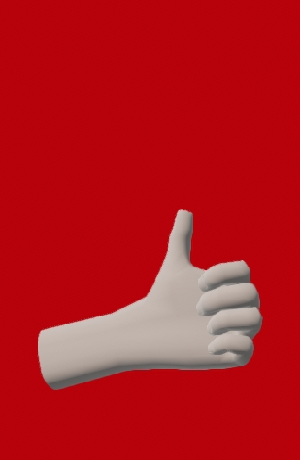
\includegraphics[width=\textwidth]{OK}
	\caption{Model: OK}
	\label{fig:modelOk}
	\end{subfigure}
	~
	\begin{subfigure}[b]{0.22\textwidth}
	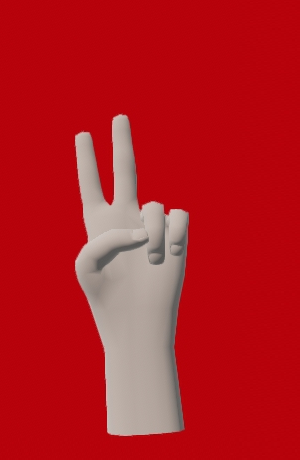
\includegraphics[width=\textwidth]{PEACE}
	\caption{Model: Pokój}
	\label{fig:modelPeace}
	\end{subfigure}
	~
	\begin{subfigure}[b]{0.22\textwidth}
	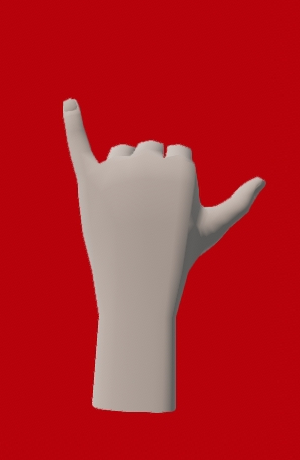
\includegraphics[width=\textwidth]{MAHALO}
	\caption{Model: Mahalo}
	\label{fig:modelMahalo}
	\end{subfigure}
	~
	\begin{subfigure}[b]{0.22\textwidth}
	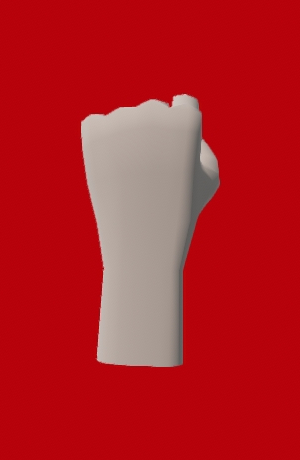
\includegraphics[width=\textwidth]{FIST}
	\caption{Model: Pięść}
	\label{fig:modelFist}
	\end{subfigure}
\caption{Modele animacji dłoni.}
\label{fig:modele}
\end{figure}
Tak jak powiedziano wcześniej, do importowania modeli używana jest wtyczka stworzona przez \textit{Google}. Jednak od tego etapu do wyświetlenia modelu na ekranie jest jeszcze kilka kroków które należy wykonać. Przede wszystkim nazwy modeli w aplikacji przechowywane są w tablicy typu \textit{String}. Niestety ten etap nie jest automatyczny, w związku z czym trzeba ręcznie podać nazwę modelu w aplikacji, aby był brany pod uwagę. Po wywołaniu funkcji \textit{renderView()}, zostaje wywołana funkcja \textit{assignModelNames()} której jedynym zadaniem jest przypisanie kolejnym pozycją w tablicy kolejnych nazw modeli z których chcemy korzystać. Nazwy te to pliki wygenerowane przez wtyczkę z rozszerzeniem \textit{.sfb}. Następnie wywoływana jest pętla w której dla każdej nie pustej nazwy w tablicy zostaje wywoływany wzorzec projektowy \textit{builder}, na klasie \textit{ModelRenderable}w celu stworzenia finałowej wersji modelu. Modele te po ``zbudowaniu`` wykorzystują klasie \textit{CompletableFuture<>} która pozwala wywołać metodę która zostanie wywołana na danym modelu gdy tylko ten zostanie ukończony. Metodą tą jest \textit{onRenderableLoades(ModelRenderable,String)} w której to modele kolejno są dodawane do zbioru przechowywanych modeli w aplikacji. Kod aplikacji~\ref{lst:loadScene} prezentuje omówione zagadnienia.
\begin{lstlisting}[caption={Generowanie sceny i modeli użytych w aplikacji.},captionpos=b,label={lst:loadScene},language = Java , frame = trBL , firstnumber = last , escapeinside={(*@}{@*)}]     
 	private void generateSceneView() {
        renderView();
        assignModelNames();

        for (String s : modelNames) {
            if (s != null && !s.equals("")) {
                ModelRenderable.builder()
                        .setSource(getContext(), Uri.parse(s))
                        .build()
                        .thenAccept(renderable -> onRenderableLoades(renderable,s))
                        .exceptionally(
                                throwable -> {
                                    Log.e("Model", "Unable to load Renderable.", throwable);
                                    return null;
                                });
            }
        }

        loadStartingModel();

        new Thread (this::startDataListener).start();
    }

    private void renderView() {
        sceneView = vw.findViewById(R.id.scene_view);
        [...]
        coreNode = new Node();
		[...]
        sceneView.getScene().addChild(coreNode);
    }                                             
\end{lstlisting}
Gdy omawiany proces zakończy się, zostaje wywołana funkcja \textit{loadStartingModel()} która jest odpowiedzialna za przygotowanie sceny, zanim dojdzie do połączenia z rękawicą kontrolerem. W funkcji tej zostaje wybrany model który zostaje przypisany do sceny jako pierwszy, a dzieję się to poprzez sprawdzanie w nowym wątku dziesięć razy na sekundę czy wybrany model został już wygenerowany przez wzorzec projektowy oraz czy został dodany do zbioru gotowych modeli. Gdy warunek ten zostanie spełniony wywoływana jest metoda \textit{setrenderable(Renderable)} która pozwala na przypisanie modelu do węzła już znajdującego się na scenie. Ostatnim elementem jest wywołanie nowego wątku w którym to ustawiany jest wysłuchiwacz zmian. Funkcja ta pokazana jest na listingu~\ref{lst:listener}. Sposób jej działanie polega na uruchomieniu nieskończonej pętli w której to są sprawdzane wartości flag zmiany danych. Flagi te są ustawiane jako prawdziwe w przypadku otrzymania nowych danych z kontrolera, co widać w ostatniej linii listingu~\ref{lst:setChar}. W ten oto sposób są sprawdzane flagi \textit{isCalibrating} co zostanie opisane w sekcji~\ref{subsec:kalibracja}, \textit{ismIsStateChanged()} dla zmian danych pochodzących z IMU z zagnieżdżonymi flagami \textit{renderRotation} oraz \textit{renderPosition}, sprawdzającymi czy użytkownik chce aby brano odpowiednio rotacji i pozycję pod uwagę podczas generowanie modelu. Działanie aplikacji w przypadku gdy te warunku są spełnione zostaną opisane odpowiednio w sekcjach~\ref{subsec:rotacja} oraz~\ref{subsec:przesuniecie}. Ostatnią flagą jest flaga pochodząca z klasy \textit{VrGlove} - \textit{ismIsFingersReadings()}, mówiąca czy dane z sensorów palców się zmieniły. 
\begin{lstlisting}[caption={Wysłuchiwacz zmian w danych rękawicy.},captionpos=b,label={lst:listener},language = Java , frame = trBL , firstnumber = last , escapeinside={(*@}{@*)}]     
private void startDataListener() {
        while(true){
            if(!isCalibrating){
                if(VrGlove.ismIsStateChanged()){
                   if(renderRotation){
                       [...]
                    if(renderPosition){
                        [...]
                }
                if(VrGlove.ismIsFingersReadings()){
                    [...]
         		}       
    }                                            
\end{lstlisting}
	
	\subsection{Rozpoznanie i animacja modelu}
	\label{subsec:rozpoznanie}
	Jeżeli dane się zmieniły od ostatniego wywołania tej funkcji wartość \\  \textit{VrGlove.ismIsFingersReadings()} zwróci prawdę co oznacza że wykona się kod rozpoznania i ewentualnej zmiany modelu. Kod ten jest obsługiwany poprzez wywołanie funkcji \textit{replaceModel()} i nie zależnie od jej działania, zawsze po jej zakończeniu wywoływana jest linia kodu \textit{VrGlove.setmIsFingersReadings(false);}, dzięki której uzyskano pewność że ten sam zestaw danych nie będzie rozpatrywany wielokrotnie -  flaga ta zostanie zmieniona na prawdziwą dopiero gdy nowe dane trafią do aplikacji. Najważniejsze kroki funkcji \textit{replaceModel()} zostaną opisane poniżej. \\
	Powiedziano wcześniej że w celu dodania nowego modelu potrzebna jest jego model, który następnie jest importowany przez plugin a nazwa zostaje dodane do tablicy w której przechowywane są nazwy modeli z rozszerzeniem \textit{.sfb}. Rzeczywiście dzięki temu model znajduję się w ramach aplikacji jednak z perspektywy użytkownika nigdy nie zostanie on zaobserwowany. Dzieję się tak z powodu ostatniego elementu który należy dodać w celu dodania nowego modelu - dla odpowiadającej mu pozycji w tablicy należy dodać tablicę pięciu liczb -1/0/1. Tablica ta odpowiednio reprezentuje pozycje palców na modelu który jest dodawany, gdzie 0 oznacza palec zgięty, 1 palec wyprostowany natomiast -1 pozycję pomiędzy tymi wygięciami. Z powodów opisanych w rozdziale~\ref{ch:rozwoj} nie zaleca się stosowania wartości -1. W ten oto sposób możemy rozpatrzeć nowe dane w kontekście istniejących modeli. \\
	W aplikacji zostały zdefiniowane wartości minimalne oraz maksymalne dla każdego sensorów. Wartości te zostały pobrane dla każdego palca gdy wszystkie palce były wyprostowane, a także gdy każdy z palców po kolei był zginany tak bardzo jak to było możliwe. Wartości te zostały pobrane eliminując wartości skrajne, czekając aż odczyty z palców się unormują wokół pewnego zakresu. W trakcie porównywania jest brany pod uwagę margines błędu rzędu $\pm 30$ wiec są to jedynie przybliżone wartości. Rezultaty tych wartości prezentuje tabela poniżej:
\begin{center}
\begin{tabular}{|c|c|c|}
\hline
Palec & Minimalna wartość & Maksymalna wartość \\ \hline
Kciuk & 520 & 680\\ \hline
Wskazujący & 400 & 580\\ \hline
Środkowy & 520 & 670\\ \hline
Serdeczny & 500 & 750 \\ \hline
Mały & 480 & 620 \\ \hline
\hline
\end{tabular}
\end{center}
Mając do dyspozycji pokazane dane, pierwszych etapem analizy sensorów palców jest sprawdzenie jak odnoszą się ona względem tych danych. Dla każdego palca następuje porównanie do wartości minimalnej oraz maksymalnej. Jeżeli wartość sensora odpowiada wartości minimalnej $\pm 30$ zostaje przypisane dla tego palca 0, w przypadku wartości maksymalnej 1 a w pozostałych przypadkach -1. Mając do dyspozycji wartości w jakiej znajduje się obecnie dłoń, oraz wymagania położenia każdego z palców w danym modelu, dokonano porównania tych stanów. Jeżeli rozpoznano model, i model ten nie jest obecnie prezentowanym modelem - funkcja zwraca nowy model który należy wygenerować. Opisany proces pokazuje listing~\ref{lst:recognize}. Generowanie nowego modelu odbywa się poprzez wywołanie funkcji \textit{assignModelToNode(ModelRenderable)}, rozpoczynając od sprawdzenia czy przekazany model posiada wartość a następnie wywołuję sekwencje zadań na wątku interfejsu. Tak jak powiedziano wcześniej model jest wyświetlany na scenie poprzez połączenie go z węzłem. Jednak aby uniknąć powtarzania tych samych sekwencji oraz zachować płynność obrazu pomiędzy głównym węzłem a modelem został dodany węzeł pośredni. Główny węzeł-rodzic odpowiada za położenie na ekranie a także rotację względem punktu początkowego. Węzeł-dziecko natomiast jest zmieniany w zależności od modelu który należy zaprezentować na ekranie. Sekwencja uruchamiana w interfejsie rozpoczyna się od utworzenia nowego węzła i przypisania mu nowego modelu, który został wybrany do prezentacji użytkownikowi.  

\begin{lstlisting}[caption={Rozpoznianie danych sensorów i wzoru modelu.},captionpos=b,label={lst:recognize},language = Java , frame = trBL , firstnumber = last , escapeinside={(*@}{@*)}]     
for (int i =0; i < fingersReadings.length; i++){
            if(fingersReadings[i] < sensorsBoundarySettings[i][0]+30.0f){
                pattern[i] = 0;
            }else if(fingersReadings[i] > sensorsBoundarySettings[i][1]-30.0f){
                pattern[i] = 1;
            }else{
                pattern[i] = -1;
            }
        }   
        for(int[] i : modelRequirements){
            for (int j = 0; j < i.length; j++){
                if(i[j] != pattern[j]){
                    break;
                }
                m = models[j];
            }
            if(m != null){
                break;
            }
        }
        if (m != null){
            if(m != currentModel){
                return m;
            }
        }
        return null;                                                        
\end{lstlisting}	
Następnie dochodzi do usunięcia obecnego modelu poprzez usunięcie ze ze sceny węzła z który model ten był powiązany a następnie dodanie węzła z nowym modelem. Cały ten proces pokazuje listing~\ref{lst:swap}, jednocześnie podsumowując proces obsługi modeli w projekcie. \newpage
\begin{lstlisting}[caption={Zamiana węzłów z powiązanymi modelami w interfejsie użytkownika.}, captionpos=b,label={lst:swap},language = Java , frame = trBL , firstnumber = last , escapeinside={(*@}{@*)}]     
Objects.requireNonNull(getActivity()).runOnUiThread(() ->{
                    Node render = new Node();
                    render.setRenderable(modelRenderable);
                    coreNode.removeChild(renderedNow);
                    renderedNow = render;
                    coreNode.addChild(render);
                    replacingInProgress = false;
        } );                                                      
\end{lstlisting}

	\subsection{Rotacja}
	\label{subsec:rotacja}
	W sekcji~\ref{subsec:rozpoznanie} pokazano w jaki sposób umiejscowiono główny węzeł na scenie prezentowanej użytkownikowi, a także w jaki sposób modele są przypisywane do węzłów pomocniczych. Tak jak wspomniano, aby model mógł się poruszać dokonywane są zmiany na węźle głównym, które jako efekt końcowy dotyczą również węzłów pomocniczych, czyli z perspektywy użytkownika - modelu dłoni. W pierwszej kolejności zostanie pokazane jak dane z IMU zostają zamienione na rotację modelu. Aby rotacja była brana pod uwagę przede wszystkim w interfejsie użytkownika przycisk typu przełącznik musi być w pozycji włączonej - oznacza to że flaga \textit{renderRotation} jest prawdziwa i aplikacja będzie dokonywała obliczeń. W tym celu wykorzystywane są dane zarówno z żyroskopu jak i akcelerometru. W pierwszej kolejności wywoływana jest funkcja \textit{calculateRotation()}, która pobiera aktualnie dostępne dane i o ile dane istnieją dla obu sensorów, zostają wywołane funkcje \textit{calculateAccAngles} oraz \textit{calculateGyroAngles}. Pierwsza z nich odpowiedzialna jest za wyliczenie kątów kontrolera na podstawie akcelerometru. W przypadku akcelerometru dla odczytów X,Y,Z, kąty te mogą zostać wyliczone dla przechyłu bocznego (ang. roll) oraz nachylenia (ang. pitch), przy użyciu następujących wzorów:
	$$
		Roll = \arctan\left(\frac{Y}{\sqrt{X^2 + Z^2}}\right)
	$$$$
		Pitch = \arctan\left(\frac{-1 * X}{\sqrt{Y^2 + Z^2}}\right)
	$$
Dzięki tym obliczeniom otrzymano wartości kątów w radianach. Aby uzyskać kąty w stopniach należy wynik przemnożyć przez \begin{Large}$\frac{180}{\pi}$\end{Large}. W ten oto sposób otrzymane kąty z akcelerometru trafiają do funkcji \textit{normalizeAngles}, która upewnia się że kąt zwracany przez \textit{Roll} nie przekroczy $\pm 85$ stopni, aby uniknąć blokady gimbala, a także w przypadku ciągłej rotacji, gdy kontroler wykona pełen obrót, czyli $360^o$, stopnie te wracają do pozycji początkowej czyli $0^o$. Jesto to zarazem końcowy efekt dla akcelerometru i wykonuję się funkcja obliczania kątów z danych żyroskopu. Jak stwierdzono w dziale~\ref{sec:oprogramowanie}, zadaniem żyroskopu w tym projekcie jest jedynie wyliczanie kątów, w związku z czym dane żyroskopy zostały zamienione na stopnie już po stronie kontrolera. Oznacza to że funkcja \textit{calculateGyroAngles} jedynie dodaje do aktualnego stanu kątów urządzenia, które w stanie początkowym wynoszą zero, nowo przesłane wyniki z żyroskopu. Kąty te następnie są normowane tak jak w przypadku akcelerometru. Końcową częścią obliczania kątów urządzenia jest zastosowanie filtra komplementarnego na podstawie obliczonych kątów z sensorów. Filtr komplementarny służy jako mechanizm kontrolowania błędu odchylenia gromadzonego przez żyroskop w długim okresie czasu, poprzez zastosowania małej korekty z bardziej dokładnego lecz wolniejszego akcelerometru. W celu skorygowania skrętu (ang. Yaw) używa się magnetometru, jednak w tym projekcie nie wykorzystano tego sensora w związku z czym jedynie dane z żyroskopu są brane pod uwagę. Poprzez ustawienie parametru filtra, można zmienić stopień w jakim akcelerometr koryguje dane - w aplikacji filtr jest ustawiony na $94\%$, co oznacza że akcelerometr koryguje dane w $6\%$. Implementacja filtra jest pokazana na listingu~\ref{lst:compFiltr}~\cite{gimbal}.
\begin{lstlisting}[caption={Implementacja filtru komplementarnego.}, captionpos=b,label={lst:compFiltr},language = Java , frame = trBL , firstnumber = last , escapeinside={(*@}{@*)}]     
float filterValue = 0.94f;
result[0] = filterValue * gyroAngles[0] + (1 - filterValue) * tmp[0];
result[1] = filterValue * gyroAngles[1] + (1 - filterValue) * tmp[1];
result[2] = gyroAngles[2];                                                    
\end{lstlisting}
W ten sposób kończy się obliczanie rotacji kontrolera według każdej z osi. Zostaje one dopasowana do orientacji dłoni na ekranie poprzez wykorzystanie zamiany kątów podanych w stopniach na kwaternion z wykorzystaniem metody \textit{axisAngle(Vector3,float)}, a następnie w celu określenia rotacji końcowej przemnożenie przez siebie poszczególnych rotacji. W mnożeniu tym ważna jest kolejność wykonywania, dlatego też jako element środkowy musi wystąpić kąt określony według osi X, który został zablokowany w przedziale $\pm 85^o$, co nie pozwala na powstanie blokady gimbala. Wynik mnożenia poszczególnych rotacji jest obrotem który należy wykonać, poprzez funkcję \textit{setLocalRotation(Quaternion)}. Przedstawiony opis algorytmu w aplikacji obsługuję rotację modelu. Proces ten pokazuje listing~\ref{lst:kwat}.
\begin{lstlisting}[caption={Obrót węzła na podstawie obliczonych kątów.}, captionpos=b,label={lst:kwat},language = Java , frame = trBL , firstnumber = last , escapeinside={(*@}{@*)}]     
Quaternion[] quat = new Quaternion[3];
calculateRotation();
quat[0] = Quaternion.axisAngle(new Vector3(0.0f,0.0f,-1.0f),modelAngles[0]); 
quat[1] = Quaternion.axisAngle(new Vector3(1.0f,0.0f,0.0f),modelAngles[1]);
quat[2] = Quaternion.axisAngle(new Vector3(0.0f,1.0f,0.0f),modelAngles[2]);
Quaternion resultOrientation = Quaternion.multiply(Quaternion.multiply(quat[1],quat[0]),quat[2]);
this.coreNode.setLocalRotation(resultOrientation);
\end{lstlisting}
	
	\subsection{Przesunięcie}
	\label{subsec:przesuniecie}	
	Ostatnim elementem zmieniającym model jest ustalenie zmiany w jego położeniu, tak aby móc odwzorować ten sam ruch na ekranie. Opcja ta gdy jest włączona, ustawia flagę \textit{renderPosition} na prawdziwą pozwalając na obliczanie pozycji. W prezentowanej aplikacji, do tego celu wykorzystywany jest tylko jedne sensor - akcelerometr. Na podstawie tych danych wylicza pozycję kontrolera funkcja \textit{parseAccDataToDisplacement()}, a następnie podobnie jak w przypadku rotacji, na głównym węźle wywoływana jest funkcja która ustawia nową pozycję. Funkcja ta to \textit{setLocalPosition(Vecotr3)}. Aby osiągnąć pozycję kontrolera na podstawie danych z akcelerometru, które są podawane w \begin{Large}
	$\frac{m}{s^2}$
	\end{Large}, należy wykonać podwójne całkowanie. Dzięki temu najpierw osiągniemy prędkość w {\Large$\frac{m}{s}$}, a następnie wartość w $m$. W tym celu podczas otrzymania nowych danych zapisywany jest czas w którym te dane pozyskano, i tak jak w przypadku danych z żyroskopu, dane te są mnożone przez upływ czasu pomiędzy pomiarami. Oczywiście wyniki z akcelerometru podlegają działaniu grawitacji, w związku z czym nie jest to jedynie prędkość poruszania się kontrolera. Wektor grawitacji jest pozyskiwany w trakcie kalibracji urządzenia co będzie opisana w sekcji~\ref{subsec:kalibracja}. Oprócz tego w prezentowanym projekcie mamy do czynienia z kontrolerem który zmienia swoją rotację, co oznacza że również wektor grawitacji zmienia się w zależności od orientacji w przestrzeni względem układu orientacji ziemi. W związku z tym aby osiągnąć prawidłowe pomiary przed całkowaniem danych, należy przywrócić pozyskane dane z orientacji w której się aktualnie znajdują, do orientacji początkowej, usunąć wektor grawitacji który w takiej pozycji pozyskano a następnie przywrócić orientację urządzenia. Dzięki temu dane które zostaną podwójnie scałkowane zwrócą wynik samego przemieszczenia bez dodatkowych sił oddziałujących na akcelerometr. W aplikacji proces ten jest osiągnięty poprzez stworzenie macierzy rotacji na podstawie obecnej orientacji modelu, dzięki której przemnożono wektor danych pozyskany z akcelerometru. Od wektora wynikowego została odjęta przechowywana grawitacja pozyskana przy kalibracji, a następnie wektor został przemnożony przez odwróconą macierz rotacji, dzięki czemu przywrócono oryginalną rotację. W ten sposób dane zostały scałkowane uzyskując pozycję. Omawiane metody prezentuje listing~\ref{lst:pos}~\cite{displacement3, displacement2, displacement}.
	\begin{lstlisting}[caption={Listing obrazujący obliczanie przemieszczenia kontrolera.}, captionpos=b,label={lst:pos},language = Java , frame = trBL , firstnumber = last , escapeinside={(*@}{@*)}]  
final float dT = (currentTime - lastTimestamp) * dtNanoToSec;
[...]	   
float[] rotationM = getRotationMatrixFromAngles(tmpAngles);
[...]
float[] accDataPostRotation = removeRotation(accSet, rotationM);
for (int i = 0; i<accDataPostRotation.length; i++ ){
	accDataPostRotation[i] -= gravityV[i];
    }
float[] invMatrix = invertMatrix(rotationM);
[...]
accDataWithoutG = multiplyMatrix3xVector(invMatrix, accDataPostRotation );
[...]
for(int i = 0; i < velocity.length; i++){
	velocity[i] += accDataWithoutG[i]*dT;
	pos[i] += velocity[i]*dT;
}
[...]
lastTimestamp = currentTime;
\end{lstlisting}
	
	\subsection{Kalibracja}
	\label{subsec:kalibracja}
	Do tej pory zostały opisane elementy sterujące animacją modelu, jego pozycją oraz orientacją, a także flagi pozwalające na wyłączenie orientacji oraz położenia. Ostatnim elementem odpowiedzialnym za zmiany na ekranie jest kalibracja modelu z kontrolerem. Dzieje się to poprzez wciśnięcie przycisku FAB na ekranie. Zmienia on wartość flagi \textit{isCalibrating}, nie pozwalając tym samym na wykonywania nowych akcji na modelu dłoni. Oprócz tego kalibracja jest wykonywana gdy nawiązano połączenie z kontrolerem oraz gdy użytkownik zmieni pozycję przycisków przełączników odpowiedzialnych za orientację i położenie. W wysłuchiwaczu przycisku FAB oprócz zatrzymania zmian na obecnie działającym modelu, resetują się wszystkie zmienne jakie do tej pory zostały pozyskane. Oznacza to że kąty modelu znów ustawione są jako zero wokół każdej osi, zmiana położenie jest liczona od nowa, ustawiony zostaje ponownie model początkowy a także jego pozycja i orientacja zostaje przywrócona do pozycji początkowej. Aby dać na dostosowanie się do tych zmian użytkownikowi, aplikacja wyświetla nowy model po upływie trzech sekund, ciągle wyświetlając przy tym wiadomość na ekranie informując użytkownika ile czasu mu się pozostało. Podczas kalibracji oczekuje się od użytkownika ustawienia lewej dłoni z wyprostowanymi palcami w taki sposób aby kciuk wskazywał ciało użytkownika a także aby utrzymać tą pozycję bez dodatkowych ruchów. Pozycja ta jest pozycją początkową modelu i to użytkownik musi się do niej zastosować. Gdy tylko kalibracja jest zakończona, pierwszym etapem przed wznowieniem pracy na ekranie jest pobranie aktualnej wartości akcelerometru - wartość ta jest pobierana przy założeniu że użytkownik nie wykonuje żadnych dodatkowych ruchów i jest zapisywana jako wektor grawitacji oddziałujący na model w pozycji kalibracyjnej. W tym momencie pozycja w jakiej się znajduje rękawica-kontrolera, jest uznawana za pozycję wyjściową, od której będą mierzone kąty obrotów wokół osi a także przemieszczenie, a modele będą się zmieniać w zależności od danych z sensorów na palcach. Wraz z opisem tej części projektu, zaprezentowano wszystkie elementy i zasady działania aplikacji wykorzystującej do działania dane z rękawicy-kontrolera.
	
	


\chapter{Dalszy rozwój projektu}
\label{ch:rozwoj}
 W rozdziałach~\ref{ch:rekawica} i ~\ref{ch:aplikacja} pokazano budowę kontrolera oraz aplikacji która wykorzystuje zbudowany kontroler w celu obsługi podstawowych funkcji rękawicy-kontrolera. Projekt ten powstał z myślą ograniczonego budżetu, prostoty wykonania oraz możliwości replikacji. Założenia te spowodowały że zdecydowano się na pewne rozwiązania które w końcowej wersji projektu pokazały swoje wady. W tym rozdziale zostanie poruszony temat błędów popełnionych w pierwszej wersji tego projektu oraz przykładowe sposoby na ich rozwiązanie w przyszłości. 
 
 \section{Problemy mikroprocesora}
 \label{sec:iuMikroprocesor}
 Przede wszystkim szukano małego mikrokontrolera tak aby nie był on przeszkodą podczas użytkowania kontrolera. O ile założenie to było dobrym pomysłem, okazało się że umiejscowienie przy brzegu sprawiło że ruch palców, w szczególności kciuka, może zmienić położenie jednostki IMU na rękawicy. Oznacza to że nawet jeśli nasza ręka znajduję się w stałej pozycji, samo poruszanie palcami wprowadza błąd w odczycie. Niestety wybór tego produktu od Arduino również przysporzył wiele kłopotów z racji błędnego rozłączania się adaptera Bluetooth. Z dotychczasowego użytkowania można stwierdzić iż kontroler poprawnie łączy się i rozłącza dwa razy, zaś w większości testowanych przypadków dochodzi do błędu połączenia przy trzeciej próbie. Aby usunąć ten błąd należy odłączyć płytkę od zasilania i podłączyć ponownie, resetując tym samym moduł. Samo oprogramowanie rękawicy skupia się na odczytach z dwóch sensorów. Praktyka pokazała że dane te nie są wystarczająco dokładne, i jeżeli to możliwe powinny być pobierane również dane magnetometru w celu dodatkowego korygowania odczytów z żyroskopu. 
 
 \section{Problemy budowy i czujników wygięcia}
 \label{sec:iuPalce}
 Problem z użytkowaniem rękawicy pojawił się dość szybko od jej zbudowania. Mianowicie wybrana do projektu rękawica była zbyt gruba, powodując dyskomfort w użytkowaniu w szczególności przez dłuższy okres czasu. Początkowe kryterium elastyczności, przesądziło o wybraniu tej rękawicy, jednak cienka rękawica również spełniła by wymagania końcowego produktu. Rozwiązanie zastosowane w celu odczytu wygięcia palców z założenia wyglądało na idealnie pasujące do wymagań projektu. Pomimo swojej prostoty wykonania oraz braku pomiaru takich cech jak odwodzenie palców czy też wygięcie poszczególnych stawów, spełnia ono swoją podstawową funkcję. Problemem tego rozwiązania jest natomiast brak elastyczności sensorów. W momencie zgięcia palców droga od knykci do paznokci się wydłuża sprawiając że sensor jest poddawany sile nacisku od strony palca która jest tym spowodowana. Sensory te pomimo braku elastyczności są zbudowane z materiału wytrzymałego na rozciąganie dzięki czemu nie pękają podczas zgięciu palców, jednak w celu zapewnienia lepszego mocowania i większej ochrony, z jednej strony została przymocowana elastyczna guma która trzyma sensor przy czubkach palców, z drugiej natomiast sensor został wszyty w rękawicę. Problem który się pojawił w trakcie użytkowania pochodził ze sposobu wszycia sensora. Została do tego użyta nić przewodząca która z powodu rozciągliwości rękawicy nie mogła zostać wszyta na sztywno, w związku z czym stawiała ona mniejszy opór podczas zginania palców i niejako została wyciągnięta przez sensor, powodując tym brak dokładności odczytów. Nić ta oprócz niskiej elastyczności okazała się być nietrwała. W trakcie korzystania z rękawicy doszło do kilku pęknięć, które zostały ponownie związane, jednak została przerwana w ten sposób ciągłość obwodu. Przez dodanie dodatkowych wiązań odczyty z sensorów się pogorszyły, sprawiając że wygięcie palca wskazującego ma większy wpływ na odczyty z kciuka, niż zgięcie kciuka samo w sobie. Podobna sytuacja przytrafiła się z sensorem małego palca oraz serdecznego. Mała powierzchnia na dłoni wokół której należało poprawić wiele połączeń, sprawiła że część nici była blisko siebie, powodując momentami odczuwalne mrowienie na dłoni. Problem ten został rozwiązany poprzez zastosowanie izolacji od wewnętrznej strony rękawicy, jednak nie gwarantuje to zwarć w obwodzie. Konkludując, nić przewodząca nie jest najlepszym rozwiązaniem w celu połączenia elementów dla tego projektu. Gdyby jednak została ona użyta, element przewodzący powinien znajdować się w środku oplotu, bądź powinny zostać zastosowane inne sposoby izolacji, a sama wytrzymałość nici powinna być znacznie większa. Mocowanie sensorów wygięcia powinno być bardziej trwałe oraz statyczne, nie pozwalając na przemieszczenie sensora na palcu. Alternatywą dla tego rozwiązania jest wykorzystanie czujników pomiaru wygięcia opartych o światło nadawane z jednej strony plastikowej tuby oraz miernika natężenia światła z drugiej. W ten sposób wiadomo że im mniejszy pomiar otrzymywanego światła, tym większe wygięcie tuby, której załamanie blokuje bezproblemowy dopływ światła. Rozwiązanie to również zapewnia pomiary niezniekształcone poprzez zachowanie innych sensorów.
 
 
  \section{Animacja modelu}
 \label{sec:iuAnimacja}
 Ostatnim elementem aplikacji dla projektu jest zapewnienie animacji dłoni. W tym celu został wykorzystany \textit{Google Sceneform}, dzięki któremu zaimportowano modele, ustawiono scenę, przypisano model a także obsługiwano przemieszczenie i orientację. Ostatnim brakującym elementem jest animacja modelu. Według dokumentacji starszej wersji projektu osiągnąć to można poprzez klasę \textit{SkeletonNode}, pozwalającą na dostęp do kości modelu, bez wykorzystania zewnętrznego programu graficznego. Jednak z niejasnych przyczyn klasa ta została usunięta w ostatniej wersji SDK, powodując brak możliwości wprowadzania zmian w modelu który został zaimportowany przy użyciu wtyczki. Problem ten rozwiązano poprzez wykorzystanie programu \textit{Blender}, dzięki któremu można było wyeksportować modele w wyznaczonej pozycji. Aby osiągnąć jednak animację modelu w czasie rzeczywistym, na podstawie dostępnych danych z sensorów wygięcia - cała klasa renderująca fragment~\ref{fig:ifceAnimacja} musi zostać napisana od nowa z wykorzystaniem innej technologii, ponieważ na oficjalnej stronie dystrybucji \textit{Sceneform}, jest napisane iż projekt został zarchiwizowany, w związku z czym taka opcja nie zostanie dodana. 
 
  \section{Błąd rotacji}
 \label{sec:iuRotacja}
 W przypadku rotacji jest wiele sposobów na polepszenie rezultatów. W prezentowanym projekcie wybrano podstawową metodę która wykorzystuje jedynie żyroskop oraz akcelerometr i przy ich użyciu wykorzystuje filtr komplementarny. Tak jak wcześniej wspomniano, aby dokładnie skorygować żyroskop na wszystkich trzech osiach, należy wykorzystać również magnetometr. Oprócz tego istnieje wiele filtrów takich jak Kalmana czy Madgwick'a które skutecznie usuwają szum, a także algorytmy wykorzystujące nowe pomiary w połączeniu z tymi zebranymi przed nimi. Możliwości łączenia technik udoskonalania odczytu rotacji z jednostek IMU sprawia, że nie ma jednego najlepszego rozwiązania, a ich wybór jest uzależniony on rodzaju projektu nad którym się pracuje. 
 
 
  \section{Problem obliczania przesunięcia}
 \label{sec:iuPrzesunięcie}
 Obliczenie położenia kontrolera w przestrzeni, niewątpliwie należy do najtrudniejszego problemu w tym projekcie. Sedno problemu tkwi w niedokładności danych. Z powodu wykorzystania metody podwójnego całkowania, błąd uzyskiwany w cm przy pojedynczej całce, rośnie do m przy całkowaniu podwójnym. Ekran aplikacji jest mierzony w m, a ruch dłoni z kontrolerem ma ograniczony zasięg długości ramienia. Pomimo tego w niedużym czasie błąd rośnie do poziomu w którym model znika z ekranu użytkownika. Niestety nie istnieje łatwy sposób na skorygowanie błędów powstałych w wyniku tego algorytmu. Firmy zajmujące tym się tym problemem dodatkowo umieszczają czujniki pozwalające określić odbiornik urządzenia i ustalić pozycję względem niego, kamery zewnętrzne obserwujące ruch w przestrzeni a także dodatkowe czujniki optyczne. W przypadku rękawicy-kontrolera który może poruszać się we wszystkich kierunkach dodatkowy problem stanowi rotacja, przez którą błąd staję się coraz większy. W przypadku prostej aplikacji nie wykorzystującej zaawansowanych jednostek pomiarowych oraz algorytmów filtrujących, często efekt jaki można osiągnąć tą techniką nie sprawdza się w zastosowaniu, dlatego też dla tej aplikacji domyślnie funkcja ta jest wyłączona. 
 
 
\chapter*{Podsumowanie}
\label{ch:podsumowanie}
\addcontentsline{toc}{chapter}{Podsumowanie}
Przedmiotem działań podjętych w celu stworzenia tej pracy było stworzenie podstawowej wersji kontrolera którego można używać w sposób intuicyjny poprzez samo poruszanie dłonią, w szczególności przeznaczonych do środowisk wirtualnej rzeczywistości. Projekt miał za zadanie przygotowanie podłoża dla dalszych prac, usprawnień a także poznania przykładowych rozwiązań znajdujących się na rynku. Podjęto działanie w celu zrozumienia problemów oraz rozwiązań nawigacji inercyjnej przy użyciu IMU, poznając zasady działania sensorów które jednostka ta obsługuje oraz standardu przesyłania tych danych poprzez adapter Bluetooth Low Energy. Został również zaadresowany problem pomiaru wygięcia palców przy niewielkim budżecie. Wszystkie te elementy zostały złożone w całość tworząc w pełni sprawny kontroler, zdolny do realizacji przedstawionych celów. Kontroler ten niestety ma też wiele wad które sprawiają że wymaga on wielu usprawnień w przyszłości. W celu poznania metod obsługi kontrolera została napisana aplikacja na system Android, pozwalająca wykorzystać stworzone urządzenie w praktyce. Wykorzystując SDK \textit{Sceneform} została przedstawiony model dłoni, reagujący na działanie kontrolera. Dedykowana aplikacja prezentuje wizualną wersję problemów nawigacji inercyjnej, pokazując skalę problemów które trzeba rozwiązać aby osiągnąć satysfakcjonujące efekty. Dzięki zebranym danym, ustalono błędy wykonane w projekcie oraz przedstawiono przykładowe sposoby na ich rozwiązanie bądź usprawnienie.  

Projekt ten pozwolił na wyciągnięcie wielu cennych lekcji dzięki zrozumieniu wszystkich jego elementów. Dzięki temu można stwierdzić że jest on niejako prototypem docelowego projektu, któremu należy poświęcić dużo więcej pracy. Mając jednak do dyspozycji odpowiednie narzędzia i budżet można osiągnąć satysfakcjonujące rozwiązanie nawet w domowych warunkach w szczególności jeżeli  poruszanym tematem jest orientacja a także kształt dłoni w czasie rzeczywistym. W celu osiągnięcia dokładnego położenia, najlepszym rozwiązaniem pozostaje jak dotąd użycie zewnętrznego systemu do śledzenia położenia. Jeżeli chcemy skorzystać z tego projektu przy użyciu dostępnych na rynku okularów VR, które posiadają w zestawie system namierzania kontrolerów, należałoby jako dodatkowy element zapewnić synchronizację, tworząc tym samym kompletny produkt w domowych warunkach. Jest to niewątpliwie projekt o dużym potencjale, z wciąż rosnącym rynkiem oraz zapotrzebowaniem i zainteresowaniem na tego typu produkty pokazywanym przez wielkie koncerny samochodowe a nawet agencje kosmiczne. Na zakończenie warto dodać że wciąż nie odkryto pełnych możliwości wirtualnej rzeczywistości, co sprawia że praca nad tym projektem jest tak ekscytująca, a na przykładzie tego projektu pokazano że nie jest to ekskluzywny rynek i każdy może w nim wziąć udział w celu zbudowania lepszej i być może wirtualnej przyszłości.  
%
%
%\addcontentsline{toc}{chapter}{Literatura}
%
\bibliographystyle{abbrv}
\bibliography{bibliografia}
%   
\listoftodos[TODOs:]
%
\end{document}